% ============================================================
% Subject Independent Multirate EMG IMU Fusion for Lower Limb
% Activity Recognition: A Reproducible Evaluation on the
% SDALLE Dataset
%
% Sections I-III are drafted content. Sections IV-X remain
% skeleton/TODO pending completed experiments (see comments).
%
% Class: IEEE Conference (official IEEEtran, conference mode)
% ============================================================
\documentclass[conference]{IEEEtran}

% ---------------------------------------------------------
% Packages (standard IEEE-conference-safe set; extend only
% as actually needed by later content)
% ---------------------------------------------------------
\usepackage{cite}
\usepackage{amsmath}
\usepackage{amssymb}
\usepackage{amsfonts}
\usepackage{algorithmic}
\usepackage{graphicx}
\usepackage{textcomp}
\usepackage{xcolor}
\usepackage{booktabs}
\usepackage{multirow}
\usepackage{url}
\usepackage{hyperref}

% Visual marker for in-manuscript TODOs so they are impossible
% to miss during drafting and trivial to grep for before
% submission (search for \todo{ or search for "TODO").
\newcommand{\todo}[1]{\textcolor{red}{\textbf{[TODO: #1]}}}

\def\BibTeX{{\rm B\kern-.05em{\sc i\kern-.025em b}\kern-.08em
    T\kern-.1667em\lower.7ex\hbox{E}\kern-.125emX}}

\begin{document}

% ---------------------------------------------------------
% Title
% ---------------------------------------------------------
\title{Subject Independent Multirate EMG IMU Fusion for Lower Limb
Activity Recognition: A Reproducible Evaluation on the SDALLE Dataset}

% ---------------------------------------------------------
% Authors and affiliations
%
% Both authors share the same institution, city, state and
% country, so that common information is stated once rather
% than repeated per author. IEEEtran's built-in \IEEEauthorrefmark
% macro renders 1/2/3/... as the symbols *, dagger, double-dagger,
% ... (it is designed for footnote-style markers, not numerals),
% so it is intentionally NOT used here. Plain \textsuperscript{}
% is used instead to get true small raised numeric superscripts
% (1, 2), which is the standard way to get numeric affiliation
% markers in an IEEEtran document. Every identifier line is
% tagged with the correct author's superscript so identifiers
% cannot be misattributed.
% ---------------------------------------------------------
\author{
\IEEEauthorblockN{Saqib Ahmad Bhat\textsuperscript{1},
P.~Subha Karuvelam\textsuperscript{2}}
\IEEEauthorblockA{
\textsuperscript{1}Department of Computer Science and Engineering\\
\textsuperscript{2}Department of Electrical and Electronics Engineering\\
\textsuperscript{1,2}Government College of Engineering, Tirunelveli, Tamil Nadu, India\\[4pt]
Email: \textsuperscript{1}\,saqibahmadbhat885@gmail.com,
\textsuperscript{2}\,subha@gcetly.ac.in\\[4pt]
\textsuperscript{1}\,\href{https://orcid.org/0009-0003-9248-6174}{https://orcid.org/0009-0003-9248-6174}\\
\textsuperscript{2}\,\href{https://orcid.org/0000-0002-9958-6106}{https://orcid.org/0000-0002-9958-6106}}
}

\maketitle

% ---------------------------------------------------------
% Abstract -- intentionally not written yet. Left as an
% explicit TODO placeholder per instruction; abstract must be
% written last, after Results and Discussion are finalized.
% ---------------------------------------------------------
\begin{abstract}
The existing benchmark for the SDALLE lower-limb EMG-IMU dataset
reports accuracies approaching 99\%, but under a window-level,
non-participant-grouped split in which the benchmark's own authors
acknowledge that windows from the same participant and trial can
appear in both training and test sets. This paper reports a
controlled, reproducible re-evaluation of SDALLE that directly
implements two directions the existing benchmark identifies as
necessary future work: strictly participant-independent evaluation
and fusion that preserves each modality's native sampling rate rather
than resampling EMG onto the IMU rate before fusion. Using nine-fold
leave-one-subject-out cross-validation, with normalization fitted
only on training participants in every fold, we compare EMG alone
(E1), IMU alone (E2), EMG-IMU fusion after resampling EMG to the IMU
rate (E3), and EMG-IMU fusion with each modality processed at its own
native rate through separate branches (E4), using an identical
convolutional architecture family across all four conditions. IMU
alone significantly outperforms EMG alone (mean accuracy
$0.679 \pm 0.063$ vs.\ $0.471 \pm 0.126$; Holm-corrected Wilcoxon
$p=0.039$). Native-rate fusion (E4) achieves the highest observed
mean accuracy ($0.716 \pm 0.074$) and macro F1 ($0.698 \pm 0.073$) of
the four conditions and is significantly better than EMG alone, but
its advantage over IMU alone and over rate-matched fusion does not
reach statistical significance after multiple-comparison correction
at this sample size ($n=9$ folds). We report this result honestly
rather than overstate it: native-rate processing is not shown to hurt
performance and produces the best point estimate, but this study does
not establish it as significantly superior to the alternatives
evaluated. All training and evaluation code, fixed random seeds, and
leakage-audit artifacts are released to support reproducibility.
\end{abstract}

\begin{IEEEkeywords}
EMG-IMU fusion, multirate sensor fusion, lower limb activity
recognition, subject-independent evaluation, leave-one-subject-out,
data leakage, reproducibility, SDALLE dataset.
\end{IEEEkeywords}

% ============================================================
% I. INTRODUCTION
% ============================================================
\section{Introduction}
\label{sec:introduction}

Automatic recognition of human movement from body-worn sensors
underpins a growing range of applications, including activity
monitoring in consumer wearables, gait and mobility assessment in
rehabilitation, control of assistive and prosthetic devices, and
quantitative biomechanics research. In each of these settings, a
system that can reliably distinguish locomotor activities such as
walking, running, and stair negotiation from streaming sensor data
provides the foundation on which higher-level analysis, such as
fall-risk estimation or exoskeleton assistance timing, is built.
The reliability of that foundation depends directly on how the
underlying recognition models are trained and, just as importantly,
on how they are evaluated before being trusted to generalize beyond
the specific people and sessions used to build them.

Two complementary sensing modalities are commonly used for
lower-limb movement recognition. Surface electromyography (EMG)
measures the electrical activity generated by muscle fibers during
contraction and therefore reflects neuromuscular activation, that
is, when and how strongly a muscle is being driven. Inertial
measurement units (IMUs), combining accelerometers and gyroscopes,
measure the resulting kinematics of the limb segment to which they
are attached, that is, how the body actually moves in space. Because
EMG activation typically precedes and shapes the kinematic response
captured by an IMU, the two signals carry related but not redundant
information about the same movement, and combining them has been
argued in prior work to improve robustness relative to using either
signal alone. We note this as a plausible and literature-supported
rationale for fusion, not as a demonstrated clinical benefit; the
present study makes no claim about clinical utility or readiness for
deployment in patient populations.

Fusing EMG and IMU streams is complicated by the fact that the two
modalities are usually sampled at different native rates: EMG must
be sampled fast enough to capture the underlying muscle action
potentials, while IMU output, being physically band-limited by body
segment motion, is typically logged at a much lower rate. Most
existing EMG-IMU pipelines resolve this mismatch by resampling one
modality onto the other, most often downsampling EMG to match the
IMU rate, before any fusion or modeling occurs. Multirate sensor
fusion, in which multiple signals with heterogeneous update rates
must be combined, is a well-studied general estimation problem
outside of activity recognition \cite{shen2022multiratefusion}, and
the choice of how to reconcile mismatched rates is known in that
literature to be a substantive design decision rather than a
formality. In EMG-IMU activity recognition specifically, this
step is nonetheless routinely applied without evaluating what, if
anything, it costs relative to processing each modality at its own
native rate.

The SDALLE dataset was introduced to support exactly this kind of
lower-limb EMG-IMU research: it provides synchronized surface EMG
and IMU recordings from nine healthy participants performing
walking, jogging, and stair ascent and descent, together with an
initial temporal convolutional network baseline
\cite{el-khoreby2025sdalle}. A subsequent benchmark study built on
the same dataset to compare sixteen deep learning architectures,
spanning feedforward, convolutional, recurrent, hybrid, and
attention-augmented designs, against a second locomotion dataset,
ENABL3S \cite{farouk2026sdalle}. That benchmark is a substantial and
useful contribution, and its authors are candid about its central
methodological limitation: the reported accuracies, which reach
approximately 99\% for attention-enhanced CNN-LSTM models on SDALLE,
come from a protocol in which normalization statistics were fitted
on the complete merged dataset before any windowing or splitting,
and in which the resulting, heavily overlapping windows were then
divided 70:30 into training and test subsets at the window level,
without grouping by participant or trial. The authors state directly
that windows from the same participant and trial can therefore
appear in both subsets, and they characterize their own reported
numbers as exploratory, protocol-specific, subject-dependent
measurements that should not be interpreted as evidence of
generalization to participants outside the training set
\cite{farouk2026sdalle}.

It is important to be precise about what is, and is not, missing
from the existing SDALLE literature. It is not the case that EMG and
IMU fusion for lower-limb recognition is unexplored; comparable
fusion pipelines have been demonstrated on other datasets, including
under participant-independent evaluation
\cite{ruhrbergestevez2025ankleexo, xu2026dsaf}. What is missing is
narrower and more specific: on SDALLE itself, neither existing study
evaluates the dataset under a protocol that is strictly independent
of participant identity, and neither examines what happens if the
two modalities are processed at their own native sampling rates
rather than resampled onto a common one before fusion. The benchmark
authors identify both points explicitly as unresolved: they
recommend, as future work, evaluation in which participant groups
are fixed before any preprocessing and normalization statistics are
fitted only on training participants, and they separately call for
approaches that pursue multi-rate fusion and retain higher-frequency
EMG information rather than discarding it through downsampling
\cite{farouk2026sdalle}. The gap this paper addresses sits precisely
at the intersection of those two, already-identified, open
questions.

This paper reports a controlled, reproducible re-evaluation of
SDALLE built around four input conditions evaluated under identical
splits: EMG alone at its native sampling rate (E1), IMU alone at its
native sampling rate (E2), EMG and IMU fused after EMG is resampled
to match the IMU rate, mirroring the approach used in the existing
benchmark (E3), and EMG and IMU fused while each modality is
processed by a separate, modality-specific branch at its own native
rate (E4). All four conditions are evaluated using nine-fold
leave-one-subject-out (LOSO) cross-validation, in which every
subject serves exactly once as the held-out test participant, and in
which normalization statistics and any other data-dependent
preprocessing decisions are fitted only on the eight training
participants in each fold, never on the held-out subject. Windows
are defined in physical time and are never allowed to cross a trial
boundary. Whether native-rate processing in E4 helps, hurts, or
makes no measurable difference relative to the rate-matched fusion
in E3 is an empirical question that this design is built to answer,
not an outcome assumed in advance; no claim about the relative
performance of E4 is made in this paper prior to the completion of
that evaluation.

In summary, this work makes four contributions, detailed fully in
Section~III: a reproducible, leakage-controlled, participant-
independent evaluation protocol for SDALLE; a controlled four-way
comparison isolating the effect of native-rate processing from the
effect of modality fusion itself; a preprocessing pipeline that
treats EMG and IMU as genuinely multirate signals rather than
collapsing them onto a single rate before modeling; and a publicly
released, reproducible implementation of the full pipeline. The
study is an empirical reproducibility and evaluation-protocol study,
not a new-architecture paper, and its conclusions are reported only
after the experiments described in Section~VI are executed.

% ============================================================
% II. RELATED WORK
% ============================================================
\section{Related Work}
\label{sec:related-work}

\subsection{EMG-Based Human Activity Recognition}
\label{subsec:emg-har}

Surface EMG has long been used for movement recognition, most
extensively for upper-limb gesture and prosthetic control, and more
recently for lower-limb locomotor activities. Zohirov et
al.~\cite{zohirov2025emglowerlimb} classified four lower-limb
movements, walking, sitting and standing, stair ascent, and stair
descent, from EMG recorded on 25 athletes using two commercial
acquisition devices. Rather than a deep network, they extracted a
compact set of time- and frequency-domain features (RMS, mean
absolute value, waveform length, zero crossings, median frequency,
and slope sign changes) and compared five classical classifiers,
finding that a Random Forest reached approximately 98.7\% accuracy
on one device and around 95\% on the other under an 80:20 random
split supplemented with cross-subject and cross-session tests. Two
points from this study are directly relevant to the present work.
First, it confirms that classical feature-based classifiers remain
competitive for EMG-only lower-limb activity classification at a
fraction of the computational cost of a deep network, which is one
reason we compare EMG-only performance explicitly as a condition
(E1) rather than assuming a fused, deep model is preferable by
default. Second, its use of cross-subject and cross-session testing,
alongside a conventional random split, illustrates that
subject-aware evaluation is already used elsewhere in EMG-based
lower-limb recognition even though it is absent from the existing
SDALLE studies. The activity set in \cite{zohirov2025emglowerlimb}
overlaps only partially with SDALLE's four classes (it does not
include jogging), and its cohort of athletic participants and
between-device accuracy gap of several percentage points also
illustrate that EMG-only performance for ostensibly similar
locomotor tasks is sensitive to acquisition hardware and population,
a caution we carry into our own interpretation of SDALLE's raw
EMG channels.

\subsection{IMU-Based Human Activity Recognition}
\label{subsec:imu-har}

IMU-based activity recognition is a considerably more mature area of
research than EMG-based recognition, reflecting the wide availability
of low-cost inertial sensors in consumer devices. Sepahvand et
al.~\cite{sepahvand2025imusurvey} survey this literature broadly,
covering sensor placement choices, feature and representation
learning approaches, and the convolutional, recurrent, and hybrid
deep learning architectures that dominate recent IMU-only pipelines.
A consistent theme in this body of work, echoed in the SDALLE
dataset paper's own per-sensor results, is that gross locomotor
activities such as walking, running, and stair negotiation are
often already highly separable from IMU kinematics alone, since
these activities differ substantially in their acceleration and
angular velocity signatures. This raises a natural question for the
present study: if IMU alone is already strong on SDALLE's four
activities, EMG's practical contribution may lie less in raising
raw classification accuracy on these particular gross activities and
more in cases requiring finer distinctions, such as effort level,
muscular fatigue, or asymmetry, that IMU kinematics alone cannot
easily resolve. We do not test such finer distinctions in this
study, since SDALLE's task definitions are limited to the four
locomotor classes; we raise the point here only to motivate why an
IMU-only condition (E2) is a necessary, not optional, baseline for
interpreting any advantage attributed to EMG or to fusion.

\subsection{Multimodal EMG-IMU Recognition}
\label{subsec:fusion-related}

Fusing EMG and IMU has been shown to be feasible under rigorous,
participant-independent evaluation on datasets other than SDALLE.
Ruhrberg Estévez et al.~\cite{ruhrbergestevez2025ankleexo} combined
eight EMG channels with three IMUs to classify five functional
lower-limb motions relevant to ankle exoskeleton control, using
leave-one-subject-out cross-validation with a small cohort of three
participants, and reported that a convolutional model adapted to an
unseen subject through few-shot calibration (ten samples per class)
reached approximately 99.3\% accuracy. Xu et
al.~\cite{xu2026dsaf} applied a dual-stream, attention-based
EMG-IMU fusion network under strict leave-one-subject-out evaluation
on the HuGaDB gait dataset (18 participants, 2 EMG and 6 IMU
channels), reporting 96.41\% accuracy with no leakage between folds.
Both studies demonstrate that EMG-IMU fusion under a genuinely
participant-independent protocol is achievable in lower-limb
locomotion and exoskeleton-control settings closely related to
SDALLE's task domain. Neither study, however, evaluates SDALLE
itself, and neither is framed around the effect of preserving native
modality sampling rates; in both cases the modalities are aligned
to a common processing rate before fusion, consistent with how the
existing SDALLE benchmark also proceeds
\cite{farouk2026sdalle}. Across the fusion literature we reviewed,
the decision of how to reconcile EMG and IMU sampling rates is
treated as a preprocessing formality rather than as an experimental
variable in its own right, which is the specific point this paper
isolates and tests.

\subsection{Subject-Independent Evaluation and Data Leakage}
\label{subsec:leakage-related}

The risk that window-level random splitting inflates reported
performance in wearable sensor-based activity recognition is
documented outside the EMG-IMU literature as well. Rehman et
al.~\cite{rehman2024validation} compared k-fold cross-validation
against leave-one-subject-out evaluation on wearable sensor data and
reported that a Random Forest classifier's accuracy dropped from
89\% under k-fold to 76\% under LOSO, a thirteen-percentage-point
gap they attribute directly to the same-subject and overlapping-
window leakage that k-fold permits and LOSO precludes; they further
note explicitly that overlap between adjacent windows compounds this
effect when combined with subject-mixed splitting. Xu et
al.~\cite{xu2026dsaf}, discussed above, show that LOSO evaluation is
both practical and already standard methodology for EMG-IMU gait
recognition on at least one comparable dataset. A preprint by
Carminati et al.~\cite{carminati2026personalization}, not yet
peer-reviewed at the time of writing, reports a considerably larger
gap on their own 11-participant, 53-class EMG-IMU gesture dataset,
with F1-score falling from 81.17\% under a standard subject-mixed
split to 20.29\% under LOSO; because that dataset involves a much
larger and more idiosyncratic gesture vocabulary than SDALLE's four
gross locomotor classes, we treat its reported magnitude as an upper
bound on what is plausible for SDALLE rather than as a directly
transferable estimate. A broader, also not yet peer-reviewed, survey
by Cai et al.~\cite{cai2025generalizablehar} situates this as a
field-wide evaluation problem in human activity recognition rather
than one specific to EMG-IMU sensing, reporting cross-person domain
shift alone can reduce accuracy by as much as 42.4\% in some of the
settings it reviews, and concluding that standardized,
leakage-aware evaluation protocols remain broadly lacking across the
field. Taken together, this literature establishes both that
window-level leakage measurably inflates reported accuracy in
activity recognition generally, and that the size of the resulting
gap is highly task- and dataset-dependent, which is precisely why
the magnitude of any such gap on SDALLE needs to be measured
directly rather than assumed from other datasets.

\subsection{SDALLE Dataset and Existing Benchmark}
\label{subsec:sdalle-related}

Two publications and one dataset record together make up the
existing SDALLE literature, and they are distinguished carefully
here because they report different things and were not equally
transparent in the same places.

The dataset was introduced by El-Khoreby et
al.~\cite{el-khoreby2025sdalle}, who recorded nine healthy
participants performing walking, jogging, and stair ascent and
descent, each reportedly repeated ten trials per activity, using
eight surface EMG channels over four muscles bilaterally and one
inertial sensor per EMG site. That paper describes acquisition
hardware as a custom sensor module relayed over Wi-Fi to a Raspberry
Pi~4 logging hub, with EMG sampling stated as supporting rates
``up to'' 2000~Hz and the inertial sensor supporting rates ``up to''
200~Hz, described as hardware capability rather than a confirmed
logged rate. Using a temporal convolutional network on this data
with wavelet-based denoising and jitter/scaling augmentation applied
to the training samples, the paper reports per-channel IMU
classification accuracies between 0.81 and 0.95 and consistently
weaker EMG-channel accuracy, which the authors attribute in part to
low EMG amplitude in their recordings. The paper does not state
whether its k-fold cross-validation groups folds by participant, and
we treat this as an open, unconfirmed point rather than assume
either answer.

A separate, later benchmark study by Farouk et
al.~\cite{farouk2026sdalle} evaluated sixteen deep learning
architectures, an ANN baseline, several CNN variants, an LSTM, and
both sequential and parallel CNN-LSTM hybrids with and without
attention, on SDALLE and, for comparison, on the independent ENABL3S
dataset. This paper reports the acquisition hardware as a DELSYS
Trigno wireless platform, with EMG logged at approximately 1259~Hz
and inertial signals logged at approximately 148~Hz, figures it
presents as the actual recorded rates rather than nominal hardware
maxima. To reconcile the resulting rate mismatch, EMG was
downsampled to the 148~Hz inertial rate using cubic interpolation,
a choice the authors justify as preserving activation timing and
envelope shape while explicitly sacrificing higher-frequency EMG
content. Data were then standardized using statistics computed from
the complete merged dataset, segmented into 16-timestep windows with
a stride of four timesteps (75\% overlap, each window spanning
approximately 0.108~s at the aligned 148~Hz rate), and split 70:30
into training and test subsets at the window level with a fixed
random seed, without grouping by participant or trial. Under this
protocol, attention-enhanced CNN-LSTM models reached accuracies
approaching 99\% on SDALLE. The authors are explicit and repeated in
stating the limits of this result: because adjacent windows share up
to twelve of sixteen samples and are split at the window level,
windows from the same participant and trial can appear in both
training and test subsets, so the reported numbers are described by
the authors themselves as exploratory, protocol-specific,
subject-dependent measurements that should not be read as evidence
of generalization to unseen participants. They further tested
WGAN-GP-based data augmentation, applied prior to the same
window-level split, and found it changed average test accuracy only
marginally (approximately 96.9\% to 96.5\%). As explicit future
work, the authors recommend fixing participant groups before any
preprocessing, fitting normalization, hyperparameter selection, and
any augmentation on training participants only, evaluating on
genuinely held-out participant windows, examining reduced window
overlap, and pursuing multi-rate fusion approaches that retain
higher-frequency EMG information rather than discarding it through
downsampling \cite{farouk2026sdalle}.

The SDALLE data itself are hosted as a public Zenodo record under a
CC-BY-4.0 license \cite{sdalle2025zenodo}, distinct from either
paper as a citable object and listing seven contributing authors
across the two papers' institutions.

Finally, we distinguish explicitly between what the two publications
report and what our own inspection of the downloaded raw SDALLE
files independently establishes, rather than silently reconciling
the two. Our raw-file audit measured native sampling rates of
approximately 1259.2593~Hz for EMG and 148.1481~Hz for IMU across
361 trials spanning the four activities and nine subjects, with 56
channels recorded per trial (8 EMG and 48 IMU, the latter consistent
with 8 sensors at 6 axes each). These measured rates numerically
match the acquisition rates reported by Farouk et
al.~\cite{farouk2026sdalle} rather than the nominal hardware maxima
reported by El-Khoreby et al.~\cite{el-khoreby2025sdalle}, but this
observation does not by itself resolve the conflicting hardware
descriptions between the two papers (a custom Raspberry-Pi-relayed
sensor module versus a named DELSYS Trigno platform); we leave that
discrepancy explicitly open rather than assume either publication is
correct. We similarly note, without further interpretation here,
that El-Khoreby et al.'s stated protocol of ten trials per activity
per subject implies 360 trials in total, one fewer than the 361
trials our audit counted; this is recorded as a minor, unresolved
discrepancy to be checked against file-level provenance before
Section~IV is finalized, not as evidence of a substantive data
quality problem. We also confirmed, only through direct inspection
and not stated explicitly in either publication, that the raw CSV
export stores the two modalities as separate multirate streams
within a single file, and that the CSV row index is not itself a
synchronized physical timestamp; our preprocessing reconstructs each
modality's native time axis separately rather than treating row
index as time, a detail described fully in Section~V.

% ============================================================
% III. RESEARCH GAP AND CONTRIBUTIONS
% ============================================================
\section{Research Gap and Contributions}
\label{sec:gap-contributions}

The gap addressed in this paper is deliberately narrow. It is not
that EMG-IMU fusion for lower-limb recognition is unexplored, since
comparable fusion pipelines have been demonstrated elsewhere, in some
cases under participant-independent evaluation
\cite{ruhrbergestevez2025ankleexo, xu2026dsaf}. It is also not that
leave-one-subject-out evaluation is a novel technique, since it is
established methodology in adjacent EMG-IMU locomotion work
\cite{xu2026dsaf} and its importance for avoiding leakage is
independently documented in the wider wearable sensing literature
\cite{rehman2024validation, cai2025generalizablehar}. Both existing
SDALLE publications are transparent that their evaluations are not
participant-independent, and the benchmark study explicitly names
two directions as necessary future work rather than as something it
attempts: evaluation with participant groups fixed before
preprocessing and normalization fitted only on training
participants, and fusion approaches that operate at each modality's
native sampling rate rather than discarding higher-frequency EMG
content through downsampling \cite{farouk2026sdalle}. The gap this
paper addresses is the intersection of those two specific,
already-identified points, applied to SDALLE: whether preserving
each modality's native sampling rate through separate,
modality-specific processing changes recognition performance,
measured under a leakage-controlled, strictly participant-independent
protocol, relative to unimodal baselines and to the rate-matched
fusion approach the existing SDALLE benchmark uses.

This paper makes four contributions.

\begin{enumerate}
\item A reproducible, leakage-controlled, participant-independent
evaluation protocol for SDALLE, using nine-fold leave-one-subject-out
cross-validation in which normalization statistics and all other
data-dependent preprocessing decisions are fitted only on training
participants in every fold, directly implementing the
participant-independent evaluation identified as necessary future
work by the existing SDALLE benchmark \cite{farouk2026sdalle}.

\item A controlled, four-condition comparison, EMG only (E1), IMU
only (E2), EMG-IMU fusion with EMG resampled to the IMU rate (E3),
and EMG-IMU fusion with each modality processed at its own native
rate through separate modality-specific branches (E4), evaluated
under identical LOSO folds, splits, and windowing rules, so that any
observed difference between E3 and E4 can be attributed to the
rate-handling choice rather than to confounding differences in data
partitioning.

\item A preprocessing pipeline that treats EMG and IMU as genuinely
multirate signals, defining windows in physical time rather than in
a fixed number of samples, reconstructing each modality's native
time axis directly from the raw acquisition files rather than from
CSV row index, and never allowing a window to cross a trial
boundary, in contrast to the single-common-rate preprocessing used
in the existing SDALLE benchmark.

\item A publicly released, reproducible implementation of the full
pipeline, comprising preprocessing, LOSO fold construction, training,
and evaluation code with fixed random seeds, together with an
explicit, code-level accounting of the specific points at which the
currently published SDALLE evaluation protocol permits train/test
leakage.
\end{enumerate}

Two boundaries on these contributions are stated explicitly. First,
this paper does not claim that native-rate processing (E4)
outperforms rate-matched fusion (E3); this is an open empirical
question that the experiments in Section~VI are designed to answer,
and the outcome, whether E4 helps, hurts, or makes no measurable
difference, is reported honestly in Sections~VII and~VIII once
those experiments are complete. Second, this paper does not claim to
be the first application of leave-one-subject-out evaluation in
EMG-IMU activity recognition, nor the first EMG-IMU fusion study;
its contribution is the first such evaluation conducted on SDALLE
specifically, combined with a controlled test of native-rate versus
rate-matched fusion that, to the literature reviewed in Section~II,
has not previously been reported for this dataset.

% ============================================================
% IV. DATASET AND SIGNAL CHARACTERISTICS
% ============================================================
\section{Dataset and Signal Characteristics}
\label{sec:dataset}

\subsection{Overview}

SDALLE consists of lower-limb locomotion recordings from nine
healthy participants performing four activity classes: walking,
jogging, stair ascent (\texttt{Stairs\_up}), and stair descent
(\texttt{Stairs\_down}) \cite{el-khoreby2025sdalle, farouk2026sdalle}.
As discussed in Sec.~II-E, the dataset paper describes a protocol of
ten trials per activity per participant, which implies a total of
360 trials. Our own file-level audit of the downloaded raw dataset,
performed by iterating over every subject and activity folder and
counting the trial CSV files actually present, identified 361 trial
files. We do not silently reconcile this difference. Locating it
precisely, the discrepancy consists of a single additional trial
file in Subject~8's walking recordings (eleven files rather than
ten); every other subject-activity combination contains exactly ten
files, as detailed in Sec.~IV-D. The additional file is retained in
our analysis because it is genuinely present in the public dataset
release, but the provenance of this specific file, for example
whether it reflects an extra recording session, a retained repeat
trial, or a file-naming artifact from data collection, is not
established by our audit and is not resolved in this manuscript.

We similarly do not resolve, and do not attempt to adjudicate, the
sensor hardware discrepancy already noted in Sec.~II-E: the dataset
paper describes a custom sensor module relayed through a Raspberry
Pi~4 Wi-Fi hub \cite{el-khoreby2025sdalle}, while the later benchmark
paper attributes acquisition to a DELSYS Trigno wireless platform
\cite{farouk2026sdalle}. Neither cited source, nor our own audit of
the distributed CSV files, establishes which description is
accurate, and we do not choose one as definitively correct. What our
audit does establish directly is the content of the files
themselves: throughout this section, sampling-rate and channel-count
figures attributed to ``our audit'' were read or computed directly
from the downloaded raw CSV files, and are reported separately from,
not as a confirmation or correction of, the hardware descriptions
given in the two publications.

\subsection{Sensor Configuration and Sampling Rates}

Every one of the 361 audited trial files contains 56 channels,
consisting of 8 surface EMG channels and 48 inertial channels. The
48 inertial channels correspond to 8 sensor locations, each
contributing 6 axes (triaxial accelerometer and triaxial
gyroscope), consistent with one EMG electrode and one inertial
sensor being co-located at each of the 8 sensing sites described in
\cite{el-khoreby2025sdalle}. This 56-channel structure was uniform
across every audited trial file, with no exceptions observed.

Each raw CSV file carries its own sampling-rate metadata, recorded
in a header row that lists a rate value for every channel. Reading
this field directly from the files, rather than deriving it from
sample counts or trial duration, our audit found a single, uniform
EMG sampling rate of approximately 1259.2593~Hz and a single,
uniform IMU sampling rate of approximately 148.1481~Hz across all
361 trials. We report these two figures as our own audit's directly
measured values; they are not quoted from either publication's
prose. They are, however, numerically consistent with the
acquisition rates Farouk et al.\ report in rounded form
(``approximately 1259~Hz'' and ``approximately 148~Hz'',
\cite{farouk2026sdalle}), and are distinct from the nominal hardware
capability figures reported by El-Khoreby et al.\ (EMG sampling
``up to'' 2000~Hz, inertial sampling ``up to'' 200~Hz,
\cite{el-khoreby2025sdalle}), which describe what the sensing
hardware supports rather than a rate confirmed to have been logged.
We do not treat either publication's figures as ground truth for
what our own audit measured; the two are reported side by side so
the reader can compare them directly.

The ratio between the two audited rates is
$1259.2593 / 148.1481 \approx 8.50$: the EMG stream advances through
approximately 8.5 samples for every one IMU sample covering the same
physical time.

\subsection{Multirate Characteristics}

The audited rate ratio in the previous subsection is the concrete
reason SDALLE is treated in this study as a genuine multirate
sensing problem rather than a dataset that merely combines two
modalities. Inspection of the raw CSV structure clarifies why. Each
file stores all 56 channels as columns of a single table, but the
row index of that table does not correspond to a shared, synchronized
physical timestamp across modalities. Every row carries a valid EMG
sample for each of the 8 EMG channels, since EMG is the
faster-updating signal, while the 48 inertial channels in that same
row hold a valid reading only once approximately every 8.5 rows, the
remaining rows carrying no inertial update, consistent with the
measured rate ratio. Reading the table row by row and treating each
row as one simultaneous EMG-IMU observation would therefore conflate
samples that occurred at different physical times for the two
modalities. This description is limited to what the distributed CSV
files themselves contain; it is not a claim about how the original
acquisition hardware performed synchronization internally, which
neither cited publication specifies in a way our audit can confirm.

Our own preprocessing addresses this directly rather than working
around it: for each trial, the EMG and inertial columns are
separated into two arrays with their own row counts (an EMG array at
the EMG sample rate and a shorter IMU array at the IMU sample rate),
and each array's time axis is reconstructed from its own known
sampling rate rather than from the shared CSV row index. This
per-modality reconstruction, not the raw file layout itself, is what
allows the two modalities to be aligned or compared on a common time
basis when required.

This distinction is what motivates comparing two fusion strategies
under an otherwise identical evaluation protocol. In E3, the EMG
stream is resampled onto the IMU's native time axis before the two
modalities are combined, mirroring the rate-matching approach used
in the existing SDALLE benchmark \cite{farouk2026sdalle}. In E4,
EMG and IMU are instead windowed independently at their own native
rates through separate, modality-specific branches, with windows
from the two modalities paired only by matching physical start time
rather than being merged onto one sampling rate beforehand. Whether
E4 offers any advantage over E3, or performs the same or worse, is
not addressed in this section and is not assumed here; it is an
empirical question evaluated in Sec.~VI and reported in Sec.~VII.

\subsection{Class Distribution and Trial Structure}

Table~\ref{tab:trial-distribution} reports the exact per-subject,
per-activity trial counts obtained by directly enumerating the trial
files in the downloaded raw dataset. Every subject-activity
combination contains exactly ten trial files with a single
exception: Subject~8's walking activity contains eleven trial files.
This is the same file responsible for the 360-versus-361 discrepancy
discussed in Sec.~IV-A; the table below simply localizes it exactly
rather than leaving it as an unlocated difference.

\begin{table}[t]
\centering
\caption{Audited trial counts per subject and activity.}
\label{tab:trial-distribution}
\begin{tabular}{lcccc}
\toprule
Subject & Jogging & Stairs\_down & Stairs\_up & Walking \\
\midrule
1 & 10 & 10 & 10 & 10 \\
2 & 10 & 10 & 10 & 10 \\
3 & 10 & 10 & 10 & 10 \\
4 & 10 & 10 & 10 & 10 \\
5 & 10 & 10 & 10 & 10 \\
6 & 10 & 10 & 10 & 10 \\
7 & 10 & 10 & 10 & 10 \\
8 & 10 & 10 & 10 & \textbf{11} \\
9 & 10 & 10 & 10 & 10 \\
\bottomrule
\end{tabular}
\end{table}

Across the nine subjects and four activities, this gives 361 trial
files in total, matching the audited total reported in Sec.~IV-A.
Trial durations are not uniform: the number of samples per trial
varies across the dataset, so each trial is treated in preprocessing
as an independently timed recording rather than assumed to span a
fixed duration.

Every trial file is treated as an independent recording unit. For
E1, E2, E3, and E4 alike, fixed-duration windows are generated by
sliding within a single trial's own signal only; no window is
constructed by concatenating or otherwise spanning two different
trial files, and no window crosses a trial boundary. Combined with
the participant-independent LOSO protocol described in Sec.~VI, this
means the trial is the smallest unit that can appear in either the
training or the held-out test partition of a given fold, never split
between the two.

% ============================================================
% V. METHODOLOGY
% ============================================================
\section{Methodology}
\label{sec:methodology}

\subsection{Preprocessing Pipeline}
\label{subsec:preprocessing}

Trial discovery follows the same enumeration used for the audit in
Sec.~IV: \texttt{dataset\_loader.py} walks every \texttt{Subject\_*}
directory, matches each subdirectory name case-insensitively against
the four canonical activity labels (\texttt{jogging},
\texttt{stairs\_down}, \texttt{stairs\_up}, \texttt{walking}), and
treats every \texttt{.csv} file found beneath a matching activity
directory as one trial. This is the identical procedure that
produced the 361-trial count reported in Sec.~IV-A, implemented once
and reused rather than re-derived.

Each raw file is parsed with a fixed line layout: the first five
lines carry file-level metadata that the pipeline does not use; line
6 is a column-header row; line 7 is the per-channel sampling-rate
row already used as the source of the rates reported in Sec.~IV-B;
and channel data begins at line 8. On every file load, the loader
re-reads line 7, extracts the first parsed EMG rate value and the
first parsed IMU rate value, and compares each against the fixed
constants 1259.2593~Hz and 148.1481~Hz with a tolerance of 1~Hz,
printing a warning (without rejecting or altering the file) if a
value falls outside that tolerance. This is a per-file consistency
check on top of the rates already reported in Sec.~IV-B, not their
original source.

The 56 columns are separated by a fixed column-index rule, not by
column name: columns $0, 7, 14, \ldots, 49$ (the first column of
each group of seven) are treated as the 8 EMG channels, and the
remaining 48 columns are treated as the IMU channels, consistent
with the 8-sensor, 7-column-per-sensor layout underlying the
channel counts in Sec.~IV-B. The EMG columns are kept for every row.
The IMU columns are then filtered by row validity: a row is kept
only if none of its 48 IMU columns is missing: measured-and-missing
values are distinguished directly in the CSV data, so no additional
threshold or heuristic is needed. Because IMU values are absent in
most rows (consistent with the roughly 8.5:1 EMG-to-IMU rate ratio
described in Sec.~IV-C), this produces one EMG array and one
strictly shorter IMU array from the same file. This row-validity
filter, not any explicit synchronization step, is the concrete
implementation-level mechanism behind the claim in Sec.~IV-C that
the CSV row index is not a shared physical timestamp: the loader
itself never reads a row as one simultaneous EMG-IMU observation. No
explicit time-axis object is constructed at this stage; each parsed
trial is stored only as a pair of plain sample arrays, one per
modality. Numeric time axes (each modality's sample index divided by
its own sampling rate) are constructed downstream, in
\texttt{windower.py}, only where they are actually needed: window
timestamps for every condition, and, for E3 only, the interpolation
described below.

No filtering or denoising step of any kind is applied to the EMG or
IMU signal values anywhere in the implemented pipeline
(\texttt{dataset\_loader.py}, \texttt{windower.py},
\texttt{normalizer.py}, \texttt{build\_datasets.py}). There is no
band-pass, low-pass, high-pass, or notch filtering; no rectification
or envelope extraction; and no wavelet or other denoising transform.
The only two operations applied to a channel's values before
per-fold normalization (Sec.~V-C) are the row-validity filtering
described above, which selects which raw IMU rows are used rather
than modifying any value, and, for the EMG stream in E3 only, the
resampling described in Sec.~V-D. Every EMG and IMU sample used
elsewhere in this pipeline is otherwise exactly the value recorded
in the raw CSV file.

Each parsed file becomes one \texttt{Trial} record carrying its
subject id, trial id, activity label, file path, and its two sample
arrays. This per-trial structure is preserved through the rest of
the pipeline: the loader never concatenates two files' arrays, the
windowing functions described next operate within a single trial's
arrays only, and, as described in Sec.~VI, whole trials, never
partial trials, are assigned to either the training or the held-out
partition of a fold. This is the code-level mechanism behind the
trial-boundary preservation already stated in Sec.~IV-D.

\subsection{Windowing Strategy}
\label{subsec:windowing}

\texttt{windower.py} fixes a 1.0\,s window length and a 0.5\,s
stride (50\% overlap) as literal constants, matching the design
already stated in Sec.~III and distinct from the 16-sample,
75\%-overlap windowing used in the window-level benchmark protocol
reviewed in Sec.~II-E, which is not used anywhere in this
implementation. From these two physical-time constants and the
audited native rates from Sec.~IV-B, the implementation computes,
once, a window length and stride in samples for each modality:
1259 EMG samples per window with a 629-sample stride, and 148 IMU
samples per window with a 74-sample stride (Table~\ref{tab:window-geometry}).
Both values are produced by truncating integer division
(\texttt{int()}) applied once when the module is loaded, not
re-derived per trial or per file.

Windows are generated by a single shared sliding function that
takes a two-dimensional sample array, a window length, and a stride:
starting at sample index 0, it repeatedly emits the slice
\texttt{[start:start+win]} together with a start/end timestamp
derived from \texttt{start} and the array's own sampling rate, then
advances \texttt{start} by the stride, and stops as soon as a full
window of length \texttt{win} no longer fits before the end of the
array. Because a window is only emitted when it fits completely,
any samples left over at the end of a trial, fewer than one window
long, are silently discarded; the implementation never pads or
emits a shorter final window. This function is invoked once per
\texttt{Trial} object and never on data spanning more than one
trial, so no window can cross a trial boundary; this is checked
directly by \texttt{sanity\_test.py}, which confirms that the final
window generated for a sampled trial ends at or before that trial's
own signal duration, not merely by design intent.

For E1 and E2, this sliding function is applied directly: E1 slides
the 1259/629 (window/stride) pair over each trial's EMG array, and
E2 slides the 148/74 pair over each trial's IMU array, each entirely
within the trial that produced it.

For E3 (described further as a fusion strategy in Sec.~V-D), each
trial's EMG stream is first resampled once, globally across the
whole trial, onto the IMU-rate time axis: a per-channel cubic
interpolant is fit over the EMG stream's own time axis
(\texttt{scipy.interpolate.interp1d}, \texttt{kind='cubic'}) and
evaluated at every IMU sample timestamp up to the shorter of the two
modalities' trial durations. The resampled 8-channel EMG array and
the original IMU array are then concatenated channel-wise into one
56-channel array, and the 148/74 (window/stride) pair is slid over
that fused array. Because the interpolation is fit once per trial
rather than once per window, every window drawn from a given trial's
fused array is built from the same trial-level interpolant.

For E4, the two modalities are windowed independently at their own
native rate rather than resampled. For each trial, the implementation
computes the number of window pairs both modalities can support,
$n_{\text{pairs}} = \min\!\big(\lfloor (n_{\text{emg}} -
1259)/629\rfloor + 1,\ \lfloor (n_{\text{imu}} - 148)/74\rfloor +
1\big)$, and, for pair $i$, slices the EMG array at
\texttt{[i$\cdot$629 : i$\cdot$629+1259]} and, independently, the
IMU array at \texttt{[i$\cdot$74 : i$\cdot$74+148]}; neither array is
resampled or interpolated. Because the EMG stride and the IMU
stride correspond to the same 0.5\,s physical stride by construction,
the $i$-th EMG window and $i$-th IMU window always begin at the same
nominal time within the trial, even though they contain a different
number of raw samples. The two per-modality window sets are returned
as two separate arrays and are never merged into one array at the
windowing stage; the only place the two modalities are combined is
inside the model itself (Sec.~V-E).

\begin{table}[t]
\centering
\caption{Window geometry and an example fold's training tensor
shape, taken directly from \texttt{windower.py} and from
\texttt{fold\_1} of each condition's generated \texttt{dataset.npz}.}
\label{tab:window-geometry}
\begin{tabular}{lcccl}
\toprule
Condition & Win. (samp.) & Stride & Ch. & Fold-1 train shape \\
\midrule
E1 (EMG)        & 1259 & 629 & 8  & $(5556,1259,8)$ \\
E2 (IMU)        & 148  & 74  & 48 & $(5564,148,48)$ \\
E3 (fused)      & 148  & 74  & 56 & $(5564,148,56)$ \\
E4 (EMG branch) & 1259 & 629 & 8  & $(5556,1259,8)$ \\
E4 (IMU branch) & 148  & 74  & 48 & $(5556,148,48)$ \\
\bottomrule
\end{tabular}
\end{table}

Table~\ref{tab:window-geometry} reports shapes from fold 1 as one
concrete example; the window length, stride, and channel count are
identical for every fold within a condition, while the exact number
of training windows varies slightly from fold to fold because a
different subject, contributing a different number of trials and
samples, is held out each time (the full per-fold LOSO construction
is described in Sec.~VI-A).

\subsection{Normalization and Leakage Prevention}
\label{subsec:normalization}

Normalization is channel-wise z-scoring, fit only on training data.
Given a training tensor of shape $(N, W, C)$ (windows, timesteps,
channels), \texttt{normalizer.py} flattens the window and timestep
dimensions together into $(N{\cdot}W, C)$ and computes one mean and
one standard deviation per channel from that flattened set; any
channel whose training-fold standard deviation is exactly zero has
its scale replaced with 1.0 to avoid division by zero. This single
fitted mean/scale pair is then applied, unchanged, to every sample
of both the training tensor and the corresponding test tensor via
$(x-\text{mean})/\text{scale}$; the test tensor is never used to
compute the mean or scale that normalizes it. For E4, two
independent scalers are fit this way, one for the EMG branch and one
for the IMU branch, so the two modalities never share normalization
statistics.

This fitting is repeated once per LOSO fold (the fold construction
itself is described in Sec.~VI-A): in \texttt{build\_datasets.py},
the training tensor passed into the normalizer is always built only
from that fold's training subjects, and the test tensor is always
built only from that fold's single held-out subject. Because a
different subject is held out in each of the nine folds, the
training-subject set, and in general the fitted mean/scale, differs
fold to fold; statistics are therefore recomputed independently for
every fold rather than fit once over the whole dataset. This is
structurally different from the protocol reviewed in Sec.~II-E, in
which normalization statistics were fitted on the complete merged
dataset before the window-level 70:30 split was applied, so that
data belonging to a test window's participant could still influence
the statistics used to normalize it. Here, no sample belonging to a
fold's held-out subject is used anywhere in computing that fold's
mean or scale. One further implementation detail worth stating
plainly: \texttt{normalizer.py} returns the fitted mean/scale pair
for each fold and branch, but \texttt{build\_datasets.py} discards
this returned value rather than saving it to disk, so the exact
per-fold statistics are reproducible by re-running the pipeline but
are not currently persisted as a separate artifact.

Table~\ref{tab:leakage-checklist} lists the specific leakage-relevant
guarantees this pipeline makes and how each is actually enforced,
rather than merely asserted in prose.

\begin{table}[t]
\centering
\caption{Leakage-prevention guarantees and how each is enforced in
the implemented pipeline.}
\label{tab:leakage-checklist}
\begin{tabular}{p{0.46\linewidth}p{0.44\linewidth}}
\toprule
Guarantee & Enforcement \\
\midrule
Held-out subject never appears in the training partition of its
own fold. &
Runtime assertion in \texttt{build\_datasets.py}
(\texttt{assert\_no\_subject\_leakage}); independently re-checked
for every fold by \texttt{sanity\_test.py}. \\[3pt]
Normalization statistics are fit only on the training partition of
a fold. &
By construction: only the training-fold tensor is passed as
\texttt{X\_train} to the normalizer. Verified empirically in
\texttt{sanity\_test.py} (normalized training set has mean
$\approx 0$, std $\approx 1$; the normalized test set is not
forced toward zero mean). \\[3pt]
No window crosses a trial boundary. &
By construction: the sliding-window function is called once per
trial and never on concatenated trials. Spot-checked in
\texttt{sanity\_test.py} by confirming a trial's final window ends
at or before that trial's own duration. \\[3pt]
Generated tensors match the declared window length and channel
count for every condition and fold. &
Runtime assertion (\texttt{assert\_shapes}) after every windowing
call in \texttt{build\_datasets.py}. \\[3pt]
E4's two branches are normalized independently rather than sharing
one statistic. &
By construction: \texttt{normalize\_dual\_branch} fits two separate
scalers, one per modality. \\
\bottomrule
\end{tabular}
\end{table}

\subsection{Fusion Strategy}
\label{subsec:fusion-strategy}

Restated at the level of what is actually passed to the model
(Sec.~V-E), the four conditions differ only in how the input tensor
or tensors for a given window are constructed. E1 supplies a single
8-channel, native-EMG-rate tensor. E2 supplies a single 48-channel,
native-IMU-rate tensor. E3 supplies a single 56-channel tensor at
the IMU rate, formed by concatenating the IMU-native window with an
EMG window built from EMG values that were resampled onto the IMU
time axis before windowing (Sec.~V-A, Sec.~V-B); this mirrors the
rate-matching approach used in the existing SDALLE benchmark
\cite{farouk2026sdalle}. E4 supplies two tensors per window pair, an
8-channel native-EMG-rate tensor and a 48-channel native-IMU-rate
tensor, with neither modality resampled or interpolated; the two
tensors are combined only inside the model (Sec.~V-E), never at the
data level.

E3 and E4 are held identical in every respect other than this
rate-handling choice: both draw from the same trial pool, the same
nine LOSO folds and the same held-out subject per fold, the same
four activity labels, and the same nominal 1.0\,s window / 0.5\,s
stride geometry; both are followed by the same per-branch
normalization procedure (Sec.~V-C) and the same encoder-and-head
model family (Sec.~V-E). What differs is only how the two
modalities' differing native rates are reconciled before
classification: E3 reconciles them before windowing, by resampling
EMG onto the IMU rate and windowing once at that common rate; E4
reconciles them after windowing, by keeping each modality at its own
rate through a modality-specific branch and combining only the
resulting feature vectors. E3's windowing is identical to E2's
(same window length, stride, and rate), and E4's EMG branch
windowing is identical to E1's, which is what makes each fusion
condition directly comparable to its corresponding unimodal
baseline.

This section documents only how each condition's input is
constructed, not which construction is more effective for
classification. Whether E4 offers any advantage over E3, no
advantage, or a disadvantage is an empirical question addressed only
in Sec.~VII, using folds that have actually been run and evaluated
under the protocol in Sec.~VI; it is not addressed, implied, or
assumed anywhere in this section.

\subsection{Models}
\label{subsec:models}

All four conditions are trained with the same small, deliberately
compact 1-D convolutional network family, defined in
\texttt{models.py} and reused unchanged in its building blocks
across conditions; only the number of input channels, and, for E4,
the number of parallel branches, changes. This is a controlled
baseline design, not a novel architecture: it composes standard
components, 1-D convolution, batch normalization, GELU activations,
max pooling, adaptive average pooling, dropout, and fully-connected
layers, in a conventional encoder-then-classifier arrangement,
chosen so that comparisons between E1--E4 are not confounded by
using materially different networks for different conditions.

Every encoder consists of two convolutional blocks in series,
separated by one 1-D max-pooling layer (kernel size 2, stride 2,
halving the sequence length). The first block maps the encoder's
input channel count to 64 output channels; the second maps 64 to
128 channels. Each block applies two successive 1-D convolutions,
each followed by batch normalization and a GELU activation: the
first convolution in a block uses kernel size 7 and the second uses
kernel size 5, both with padding equal to half the kernel size (so
that sequence length is unchanged by the convolutions themselves;
length reduction comes only from the pooling layers), and both omit
an explicit bias term, relying on the following batch-normalization
layer instead. After the second block, an adaptive average-pooling
layer collapses whatever time dimension remains to a single value
per channel, yielding a fixed-length 128-dimensional feature vector
regardless of how many timesteps the encoder received as input; this
is what allows E1's 1259-sample windows and E2/E3's 148-sample
windows to be processed by architecturally identical encoders that
differ only in input channel count and produce equal-length output
vectors.

The classification head is shared in design across all four
conditions: a linear layer to a 64-dimensional hidden representation,
a GELU activation, a dropout layer (rate 0.3, the only dropout in
the network, and a fixed part of the model definition rather than a
training-time choice), and a final linear layer to 4 output logits,
one per activity class in the same order used throughout this paper
(jogging, stairs\_down, stairs\_up, walking). The head returns raw
logits with no softmax or other output normalization; the predicted
class used at evaluation time (Sec.~VI) is the argmax over these
four logits.

E1, E2, and E3 use a single-branch model: one encoder followed by
one head taking the encoder's 128-dimensional output. The only
difference between the three is the encoder's input channel count,
fixed by the input construction in Sec.~V-D: 8 for E1, 48 for E2,
and 56 for E3. E4 uses a dual-branch model: two encoders that share
no weights, one with an 8-channel input processing the EMG branch
and one with a 48-channel input processing the IMU branch, each
independently producing its own 128-dimensional feature vector. The
two feature vectors are concatenated into one 256-dimensional
vector, which is then passed to a head sized for that width. This
channel-wise concatenation, performed once per forward pass after
both encoders have already run to completion, is the only point at
which E4 combines the two modalities; no other feature-level or
decision-level fusion mechanism is used.

All four models expect input in PyTorch's (batch, channels,
timesteps) convention, while the tensors produced by the pipeline in
Sec.~V-A--V-D are stored as (windows, timesteps, channels); this
axis transpose is applied by the training and evaluation code
described in Sec.~VI, not inside \texttt{models.py} itself.

Model capacity is not held equal across the four conditions, and we
report this rather than assume it. Counting trainable parameters
directly from each instantiated model (summing
\texttt{p.numel()} over every parameter with
\texttt{requires\_grad=True}), and cross-checked as identical across
folds of the same condition since the architecture does not depend
on which subject is held out, the four models contain 156{,}228
(E1), 174{,}148 (E2), 177{,}732 (E3), and 330{,}052 (E4) trainable
parameters. The differences are structural, not incidental: the
leading convolutional layer's parameter count scales with the
number of input channels (8, 48, and 56 for E1, E2, and E3
respectively), and E4 instantiates two complete, separately
parameterized encoders rather than one, together with a wider first
head layer that accepts the concatenated 256-dimensional feature
vector rather than the 128-dimensional vector used by the
single-branch models. We do not claim equal model capacity across
E1--E4; the encoder-and-head design family is identical, but its
size is not, and any performance difference reported in Sec.~VII
should be read with this capacity asymmetry in mind rather than
attributed only to whether fusion is rate-matched or native-rate.

% ============================================================
% VI. EXPERIMENTAL PROTOCOL
% ============================================================
\section{Experimental Protocol}
\label{sec:protocol}

\subsection{Leave-One-Subject-Out Protocol}
\label{subsec:loso}

The evaluation protocol is nine-fold leave-one-subject-out,
implemented in \texttt{build\_datasets.py}. The nine subject ids
identified in the audit (Sec.~IV-A) are enumerated once; for each
subject in turn, that subject's trials alone form the held-out test
partition of one fold, and every other subject's trials form that
fold's training partition. Every subject therefore serves exactly
once as the held-out test subject, and every fold has eight training
subjects and one test subject. Before saving a fold, the
implementation runs a runtime assertion that the held-out subject id
is absent from the training-subject id set and that the test
partition contains only that one subject; the presence of all nine
folds for all four conditions under \texttt{data/processed/} is
evidence that this assertion passed for every fold actually built,
since the script raises immediately and does not write a fold's
output if it fails. This construction is repeated independently for
each of E1--E4, using the windowing rules described in Sec.~V-B, so
all four conditions share the same nine train/test subject splits.

Isolation is enforced at the level of whole trials, not merely
subjects: because a trial is assigned in its entirety to either the
training or the test partition of a fold (Sec.~V-A), and windows are
generated only within a single trial's own signal (Sec.~V-B), no
window can be built from samples spanning both partitions. We do not
claim any stronger isolation than this: the implementation does not
control for, or report on, any other property of the split, such as
balancing activity counts or session order between partitions beyond
what naturally follows from holding out one subject's trials at a
time.

Normalization statistics are fit only on each fold's training
partition and applied unchanged to that fold's test partition,
exactly as described in Sec.~V-C; we do not repeat that description
here. One point is stated plainly, including its own history, because
it bears directly on how the training configuration in Sec.~VI-C
should be read: the implementation does not carve out a separate
validation subject distinct from the held-out test subject, and no
such third partition exists anywhere in this protocol. An earlier
version of \texttt{train.py} computed per-epoch loss and accuracy on
the held-out test fold and used that value to drive the
learning-rate scheduler; this is a source of test-set influence on
the training process, since the one partition this protocol reports
performance on would also have been shaping optimization. This was
identified during development, before any of the final training runs
reported in Sec.~VI-C were produced, and was corrected in
\texttt{train.py}: in the corrected implementation actually used for
every run reported in this paper, the held-out test fold is not read
at any point inside the epoch loop, no test loss, test accuracy, or
other test-derived signal is computed during training, and the
learning-rate scheduler (Sec.~VI-C) is driven by training loss only.
Correspondingly, the hyperparameters reported in Sec.~VI-C are not
the product of any search or validation procedure at all: they are
fixed constants set once in \texttt{train.py} before training, and we
make no claim that they were tuned or selected using a held-out
validation set.

\subsection{Replication Check Against the Published Protocol}
\label{subsec:replication-check}

We checked the project source code directly for an implementation of
the window-level, non-participant-independent 70:30 split protocol
used in the existing SDALLE benchmark \cite{farouk2026sdalle} (Sec.~II-E),
which would provide a sanity-check replication baseline separate
from the LOSO results. No such implementation exists anywhere in
\texttt{src/}, and no output, log, or saved artifact corresponding
to a window-level 70:30 split run was found anywhere in the project.
A faithful replication check against the published protocol was
therefore not performed in this project. We state this directly
rather than implying otherwise, and no replication result is
reported anywhere in this manuscript.

\subsection{Hyperparameters and Training Configuration}
\label{subsec:hyperparameters}

Training is implemented in \texttt{train.py} and uses a fixed set of
hyperparameters, defined once as constants rather than searched or
tuned: the Adam optimizer with learning rate $1\times10^{-3}$ and
weight decay $1\times10^{-4}$; a batch size of 64 for both the
training and evaluation data loaders (the training loader shuffles
batches each epoch, \texttt{shuffle=True}; the evaluation loader
does not, \texttt{shuffle=False}); and the standard multi-class
cross-entropy loss (\texttt{torch.nn.CrossEntropyLoss}), used
unweighted, with no class-weighting term passed to it. (The module's
own header comment mentions an optional \texttt{--weighted} flag for
class-weighted loss; no such command-line argument or code branch
actually exists in \texttt{train.py}, so this description in the
comment does not correspond to any executable behavior, and no class
weighting was applied in any run.) A learning-rate scheduler,
\texttt{ReduceLROnPlateau} (mode \texttt{"min"}, patience 5, factor
0.5), is stepped once per epoch using that epoch's training loss. As
described in Sec.~VI-A, the scheduler is driven by training loss
because no validation partition was used in this protocol: the
held-out test subject was not used for optimization, scheduling,
checkpoint selection, or hyperparameter selection in any of the
training runs reported below. No early-stopping criterion is
implemented: every run executes the full requested number of epochs
regardless of training-loss behavior; there is no validation-based
stopping rule, and none is claimed. No gradient clipping is applied.
No data augmentation of
any kind is implemented anywhere in the pipeline. The random seed is
fixed at 42 and reset at the start of every fold's training run via
a dedicated function that seeds Python's \texttt{random}, NumPy, and
PyTorch (including \texttt{torch.cuda.manual\_seed\_all} when a CUDA
device is available), and additionally sets
\texttt{torch.backends.cudnn.deterministic=True} and
\texttt{cudnn.benchmark=False}, settings that only affect behavior
if a CUDA GPU is the device in use. Model weights are saved once,
after the full epoch loop for a fold completes
(\texttt{model.state\_dict()} to \texttt{model.pt}); there
is no best-epoch checkpoint selection based on validation
performance, since only the final epoch's weights are ever written.

The number of epochs actually run is uniform across every condition
and fold in the results reported in this paper, and we state the
route by which that came to be true rather than only the end state.
Two earlier, non-final rounds of training exist in the project's
history and are not the basis for anything reported in Sec.~VII:
an initial partial run trained E1 for the full 50 epochs on folds 1
through 7 only (folds 8 and 9 untrained), together with a 3-epoch
smoke test of fold 1 for E2, E3, and E4, and both of these predate
the scheduler correction described in Sec.~VI-A. After that
correction, every one of the 36 (experiment, fold) combinations,
E1--E4 crossed with folds 1--9, was retrained from a freshly
initialized model under the corrected protocol, for the full 50
epochs, with the random seed fixed at 42 as described above. The
saved per-fold metadata
(\texttt{results/<EXP>/fold\_<N>/meta.json}) confirms 50 epochs and
seed 42 for all 36 folds, and \texttt{results/experiment\_manifest.csv}
records a \texttt{COMPLETE} status, parameter count, training and
inference time, and hyperparameters for each. SHA-256 checksums of
all 36 \texttt{model.pt} files were computed and stored in
\texttt{results/final\_results\_checksums.sha256}, and a full copy of
\texttt{results/} was preserved to \texttt{results\_backup/}
immediately after training, before evaluation (Sec.~VI-D) was run;
this is what allows Sec.~VI-D to load and verify each model's weights
against a fixed, recorded checksum rather than trusting that the file
on disk is unchanged. No fold's checkpoint was retrained,
overwritten, or renamed after this point. Total measured training
time across all 36 folds was approximately 18.0~hours
(E1: 2170~s; E2: 345~s; E3: 337~s; E4: 61{,}996~s, summed over 9
folds each), computed directly from the per-fold \texttt{train\_time\_s}
values in \texttt{meta.json}; per-fold timing is reported here only
as a record of what was measured; it is not a claim about the
relative computational cost of the four architectures.

\subsection{Evaluation Metrics and Statistical Analysis}
\label{subsec:eval-metrics}

Evaluation is implemented in \texttt{evaluate.py}. For a trained
fold, it loads the corresponding saved model and that fold's test
partition, runs inference with the model in evaluation mode (no
gradient computation), and computes, from a directly constructed
$4\times4$ confusion matrix rather than a third-party metrics
library: overall accuracy, macro-averaged precision, recall, and
F1, per-class precision, recall, and F1 for each of the four
activity classes, and the confusion matrix itself. When more than
one fold is evaluated in a single run, per-fold metrics are reported
individually together with an aggregate confusion matrix and
aggregate metrics pooled across all evaluated folds' predictions.
These are the only metrics implemented; no other evaluation
criterion exists in the code.

The per-fold metrics just described are computed identically by two
scripts at different stages of the project: \texttt{evaluate.py},
used during development, and \texttt{run\_evaluation.py}, a later,
self-contained evaluation pipeline that reimplements the same
confusion-matrix-based metric computation and is the script whose
output is the source of every number reported in Sec.~VII. Before
running any inference, \texttt{run\_evaluation.py} recomputes the
SHA-256 checksum of every \texttt{model.pt} file and compares it
against the fixed values recorded in
\texttt{results/final\_results\_checksums.sha256} (Sec.~VI-C),
raising an error rather than proceeding if any checkpoint's checksum
does not match; it does not retrain any model, does not refit
normalization, and reads test tensors directly from each fold's
already-built \texttt{dataset.npz} (Sec.~V-C).

Beyond per-fold metrics, \texttt{run\_evaluation.py} additionally
implements an inferential statistical comparison across the four
conditions, which no earlier version of the codebase contained.
For each of the six unordered pairs among E1--E4, it computes a
two-sided Wilcoxon signed-rank test (\texttt{scipy.stats.wilcoxon})
treating the nine LOSO folds as paired observations, since the same
nine train/test splits (Sec.~VI-A) are shared across all four
conditions; this is done separately for per-fold accuracy and for
per-fold macro F1. The resulting six raw $p$-values are corrected
for multiple comparisons within each metric using the
Holm--Bonferroni step-down procedure, and a paired Cohen's $d$
(mean of the paired differences divided by their sample standard
deviation) is reported alongside each comparison as an effect-size
measure independent of the correction. The statistical unit
throughout is the subject-fold ($n=9$ per condition), not the
individual window, precisely to avoid treating temporally correlated
windows from the same held-out subject as independent observations;
this was flagged as a limitation on statistical power when no test
existed at all, and the same $n=9$ constraint still applies now that
the test has been implemented and run, and is discussed further in
Sec.~IX.

We also report evaluation coverage precisely, since it is not always
one-to-one with training coverage in this project's history. As
currently saved, \texttt{evaluation/evaluation\_manifest.csv} and
\texttt{evaluation/final\_metrics.csv} record all 36
(experiment, fold) combinations, E1--E4 crossed with folds 1--9, as
evaluated exactly once, each against the retrained, checksum-verified
model described in Sec.~VI-C; the pre-correction partial and
smoke-test checkpoints mentioned there were never evaluated and are
not the source of any reported number. Every metric, table, and
figure in Sec.~VII is traceable to
\texttt{evaluation/final\_metrics.csv}, the four
\texttt{evaluation/metrics/<EXP>\_summary.json} files, or
\texttt{evaluation/metrics/statistical\_tests.json}.

\subsection{Computational Environment}
\label{subsec:compute-env}

We report only what can be established directly from artifacts in
the project, and say so explicitly where something cannot be
established, rather than estimate it. An earlier version of this
subsection reported that the environment used to produce the trained
models could not be established at all, because the project's
checked-in virtual environment (\texttt{.venv}, Python 3.13.12) did
not contain a PyTorch installation. That gap has since been closed
for the final training run reported in Sec.~VI-C: the orchestration
script (\texttt{run\_all.sh}) that launched all 36 retrained folds
records its own environment at the start of the run, in
\texttt{results/final\_training.log}, giving Python 3.13.12 and
PyTorch 2.14.0, with the \texttt{--device} argument (Sec.~VI-C) fixed
to \texttt{"mps"}, PyTorch's Apple GPU (Metal Performance Shaders)
backend, for every one of the 36 folds. The run completed on
3~September~2026 (timestamps recorded in
\texttt{results/final\_training.log} and in every fold's
\texttt{meta.json}). We do not have an independently logged operating
system version or hardware model beyond what MPS availability
implies (a Mac running a PyTorch-MPS-capable macOS version on Apple
silicon); no artifact in the project records either more precisely,
and we do not guess at them.

Across the files actually imported by the pipeline, the only
third-party packages used anywhere in \texttt{src/} are NumPy,
SciPy (only \texttt{scipy.interpolate.interp1d}, in
\texttt{windower.py}, and, in \texttt{run\_evaluation.py} only,
\texttt{scipy.stats.wilcoxon} for the statistical comparisons in
Sec.~VI-D), and PyTorch (in \texttt{models.py}, \texttt{train.py},
\texttt{evaluate.py}, and \texttt{run\_evaluation.py}); no script in
\texttt{src/} imports scikit-learn or pandas, even though both
appear in \texttt{requirements.txt}. We do not have a logged version
number for the specific SciPy build used at evaluation time, and
report only that it is the SciPy installed in the same environment
whose Python and PyTorch versions are given above.

One further observation follows directly from the per-fold timing
recorded in \texttt{meta.json} and is reported for completeness
rather than interpreted causally: measured training time per fold
was far from uniform across conditions. E2 and E3 folds each
completed in tens of seconds, E1 folds in a few hundred seconds, and
every E4 fold took substantially longer, from just under two hours
to just over three hours. We report this difference because it is
directly measurable from the saved metadata, not because we have run
a controlled comparison that isolates its cause; plausible
contributors include E4's larger parameter count (Sec.~V-E) and
known variability in PyTorch's MPS backend for some multi-input
model patterns, but we did not test either explanation directly, and
no timing claim in this subsection should be read as a statement
about the relative computational cost of native-rate versus
rate-matched fusion in general, only about what was measured in this
specific run.

% ============================================================
% VII. RESULTS
% ============================================================
\section{Results}
\label{sec:results}

All numbers, tables, and figures in this section are computed by
\texttt{run\_evaluation.py} from the 36 retrained, checksum-verified
model checkpoints described in Sec.~VI-C, over all nine LOSO folds of
all four conditions (Sec.~VI-D); none are estimated, interpolated, or
carried over from the earlier partial or smoke-test runs mentioned in
Sec.~VI-C. Reported means and standard deviations are taken across
the nine per-fold values for a given condition unless stated
otherwise.

\subsection{Overall Performance}
\label{subsec:results-overall}

Table~\ref{tab:overall-performance} reports mean, standard deviation,
and median accuracy and macro F1 for each condition, and
Fig.~\ref{fig:summary-bar} shows the same means and standard
deviations graphically. Ordered by mean accuracy, EMG alone (E1) is
lowest at $0.471 \pm 0.126$, IMU alone (E2) reaches $0.679 \pm 0.063$,
rate-matched fusion (E3) reaches $0.634 \pm 0.139$, and native-rate
multirate fusion (E4) is highest at $0.716 \pm 0.074$; macro F1 shows
the same ordering (E1 $0.378$, E3 $0.622$, E2 $0.665$, E4 $0.698$),
with E2 and E3 swapping places relative to accuracy because E3's
substantially higher fold-to-fold variability (Sec.~VII-D) pulls its
mean down more under F1, which weights every class equally, than
under accuracy, which does not. E4 achieves the highest observed mean
on both metrics. Whether this ordering reflects statistically
reliable differences, as opposed to differences that could plausibly
arise from fold-to-fold variability alone, is addressed directly in
Sec.~VII-E and is not assumed here from the means alone.

\begin{table}[t]
\centering
\caption{Overall performance across nine LOSO folds. Values are
mean $\pm$ standard deviation, with median in parentheses.}
\label{tab:overall-performance}
\begin{tabular}{lcc}
\toprule
Condition & Accuracy & Macro F1 \\
\midrule
E1 (EMG only)        & $0.471 \pm 0.126$ (0.452) & $0.378 \pm 0.123$ (0.353) \\
E2 (IMU only)        & $0.679 \pm 0.063$ (0.662) & $0.665 \pm 0.063$ (0.648) \\
E3 (rate-matched)    & $0.634 \pm 0.139$ (0.690) & $0.622 \pm 0.129$ (0.678) \\
E4 (native-rate)     & $0.716 \pm 0.074$ (0.709) & $0.698 \pm 0.073$ (0.712) \\
\bottomrule
\end{tabular}
\end{table}

\begin{figure}[t]
\centering
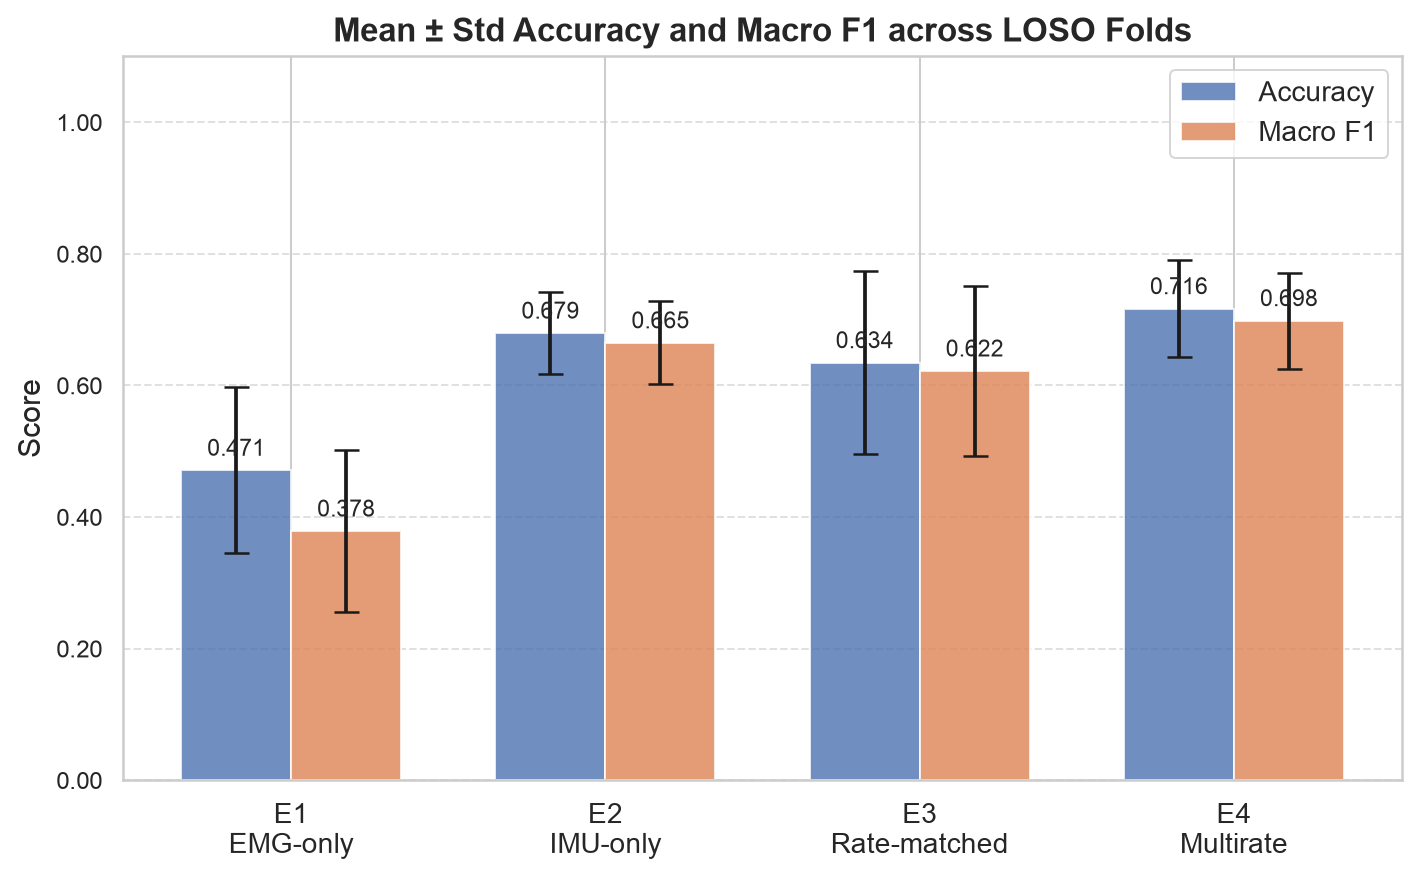
\includegraphics[width=\linewidth]{figures/summary_bar.png}
\caption{Mean accuracy and macro F1 across the nine LOSO folds for
each condition, with error bars showing one standard deviation. Same
values as Table~\ref{tab:overall-performance}.}
\label{fig:summary-bar}
\end{figure}

\subsection{Per-Activity Performance}
\label{subsec:results-per-activity}

Table~\ref{tab:per-class-f1} reports per-class F1, pooled across all
test windows from all nine folds of each condition (that is, computed
from each condition's aggregate confusion matrix, not averaged
across folds), for the four activity classes. Two patterns are
consistent across all four conditions: walking is recognized at least
as well as, and usually better than, the other three classes, and
stair ascent (\texttt{Stairs\_up}) is the hardest class for every
condition except E2. The pattern is most extreme for E1: aggregate
recall for \texttt{Stairs\_up} is only $0.143$ (precision $0.431$),
far below its recall for walking ($0.695$), meaning EMG alone
correctly identifies stair ascent in barely one attempt out of seven
in this pooled sense, while most of the missed \texttt{Stairs\_up}
windows are predicted as \texttt{Stairs\_down} (Sec.~VII-C). Adding
IMU, whether rate-matched (E3) or native-rate (E4), raises
\texttt{Stairs\_up} recall substantially, to $0.539$ and $0.656$
respectively, though it remains the lowest-recall class for both
fusion conditions. \texttt{Stairs\_down} shows the opposite
precision/recall imbalance under E3 specifically: precision is only
$0.425$ against a recall of $0.658$, indicating that E3 over-predicts
\texttt{Stairs\_down} relative to its true frequency, a pattern not
present to the same degree in E2 or E4.

\begin{table}[t]
\centering
\caption{Per-class F1, pooled across all test windows of all nine
folds for each condition. Full precision/recall breakdowns are in
\texttt{evaluation/metrics/*\_summary.json}.}
\label{tab:per-class-f1}
\begin{tabular}{lcccc}
\toprule
Condition & Jogging & Stairs\_down & Stairs\_up & Walking \\
\midrule
E1 & 0.484 & 0.326 & 0.215 & 0.612 \\
E2 & 0.696 & 0.573 & 0.636 & 0.733 \\
E3 & 0.722 & 0.516 & 0.599 & 0.670 \\
E4 & 0.755 & 0.617 & 0.685 & 0.749 \\
\bottomrule
\end{tabular}
\end{table}

\subsection{Confusion Matrices}
\label{subsec:results-confusion}

Fig.~\ref{fig:confusion-matrices} shows the row-normalized aggregate
confusion matrix for each condition, so that each row sums to 1 and
the diagonal entries equal the per-class recall reported in
Sec.~VII-B. The matrices make the source of E1's weak
\texttt{Stairs\_up} recall visible directly: 36\% of true
\texttt{Stairs\_up} windows are misclassified as \texttt{Stairs\_down}
and a further 27\% as walking, so EMG-only confuses stair ascent with
both the visually and physiologically related stair-descent activity
and, more surprisingly, with level walking, more often than it
identifies it correctly. \texttt{Stairs\_down} is itself E1's
second-weakest class (recall $0.338$), with 40\% of its true windows
predicted as walking; jogging and walking are comparatively well
separated from each other in E1 (at most 17--18\% mutual confusion in
either direction). Adding IMU sharpens every diagonal substantially:
in E2, E3, and E4 alike, the two stair classes remain the most
mutually confusable pair in the matrix (for example, E4 confuses
9--12\% of \texttt{Stairs\_down} and \texttt{Stairs\_up} windows with
each other in each direction), consistent with these two activities
sharing similar limb kinematics that differ mainly in gravity-relative
direction, a distinction IMU-derived orientation and acceleration
cues resolve only partially. Jogging and walking remain the most
cleanly separated pair under every condition that includes IMU, with
E4 reaching 75--77\% recall on each.

\begin{figure}[t]
\centering
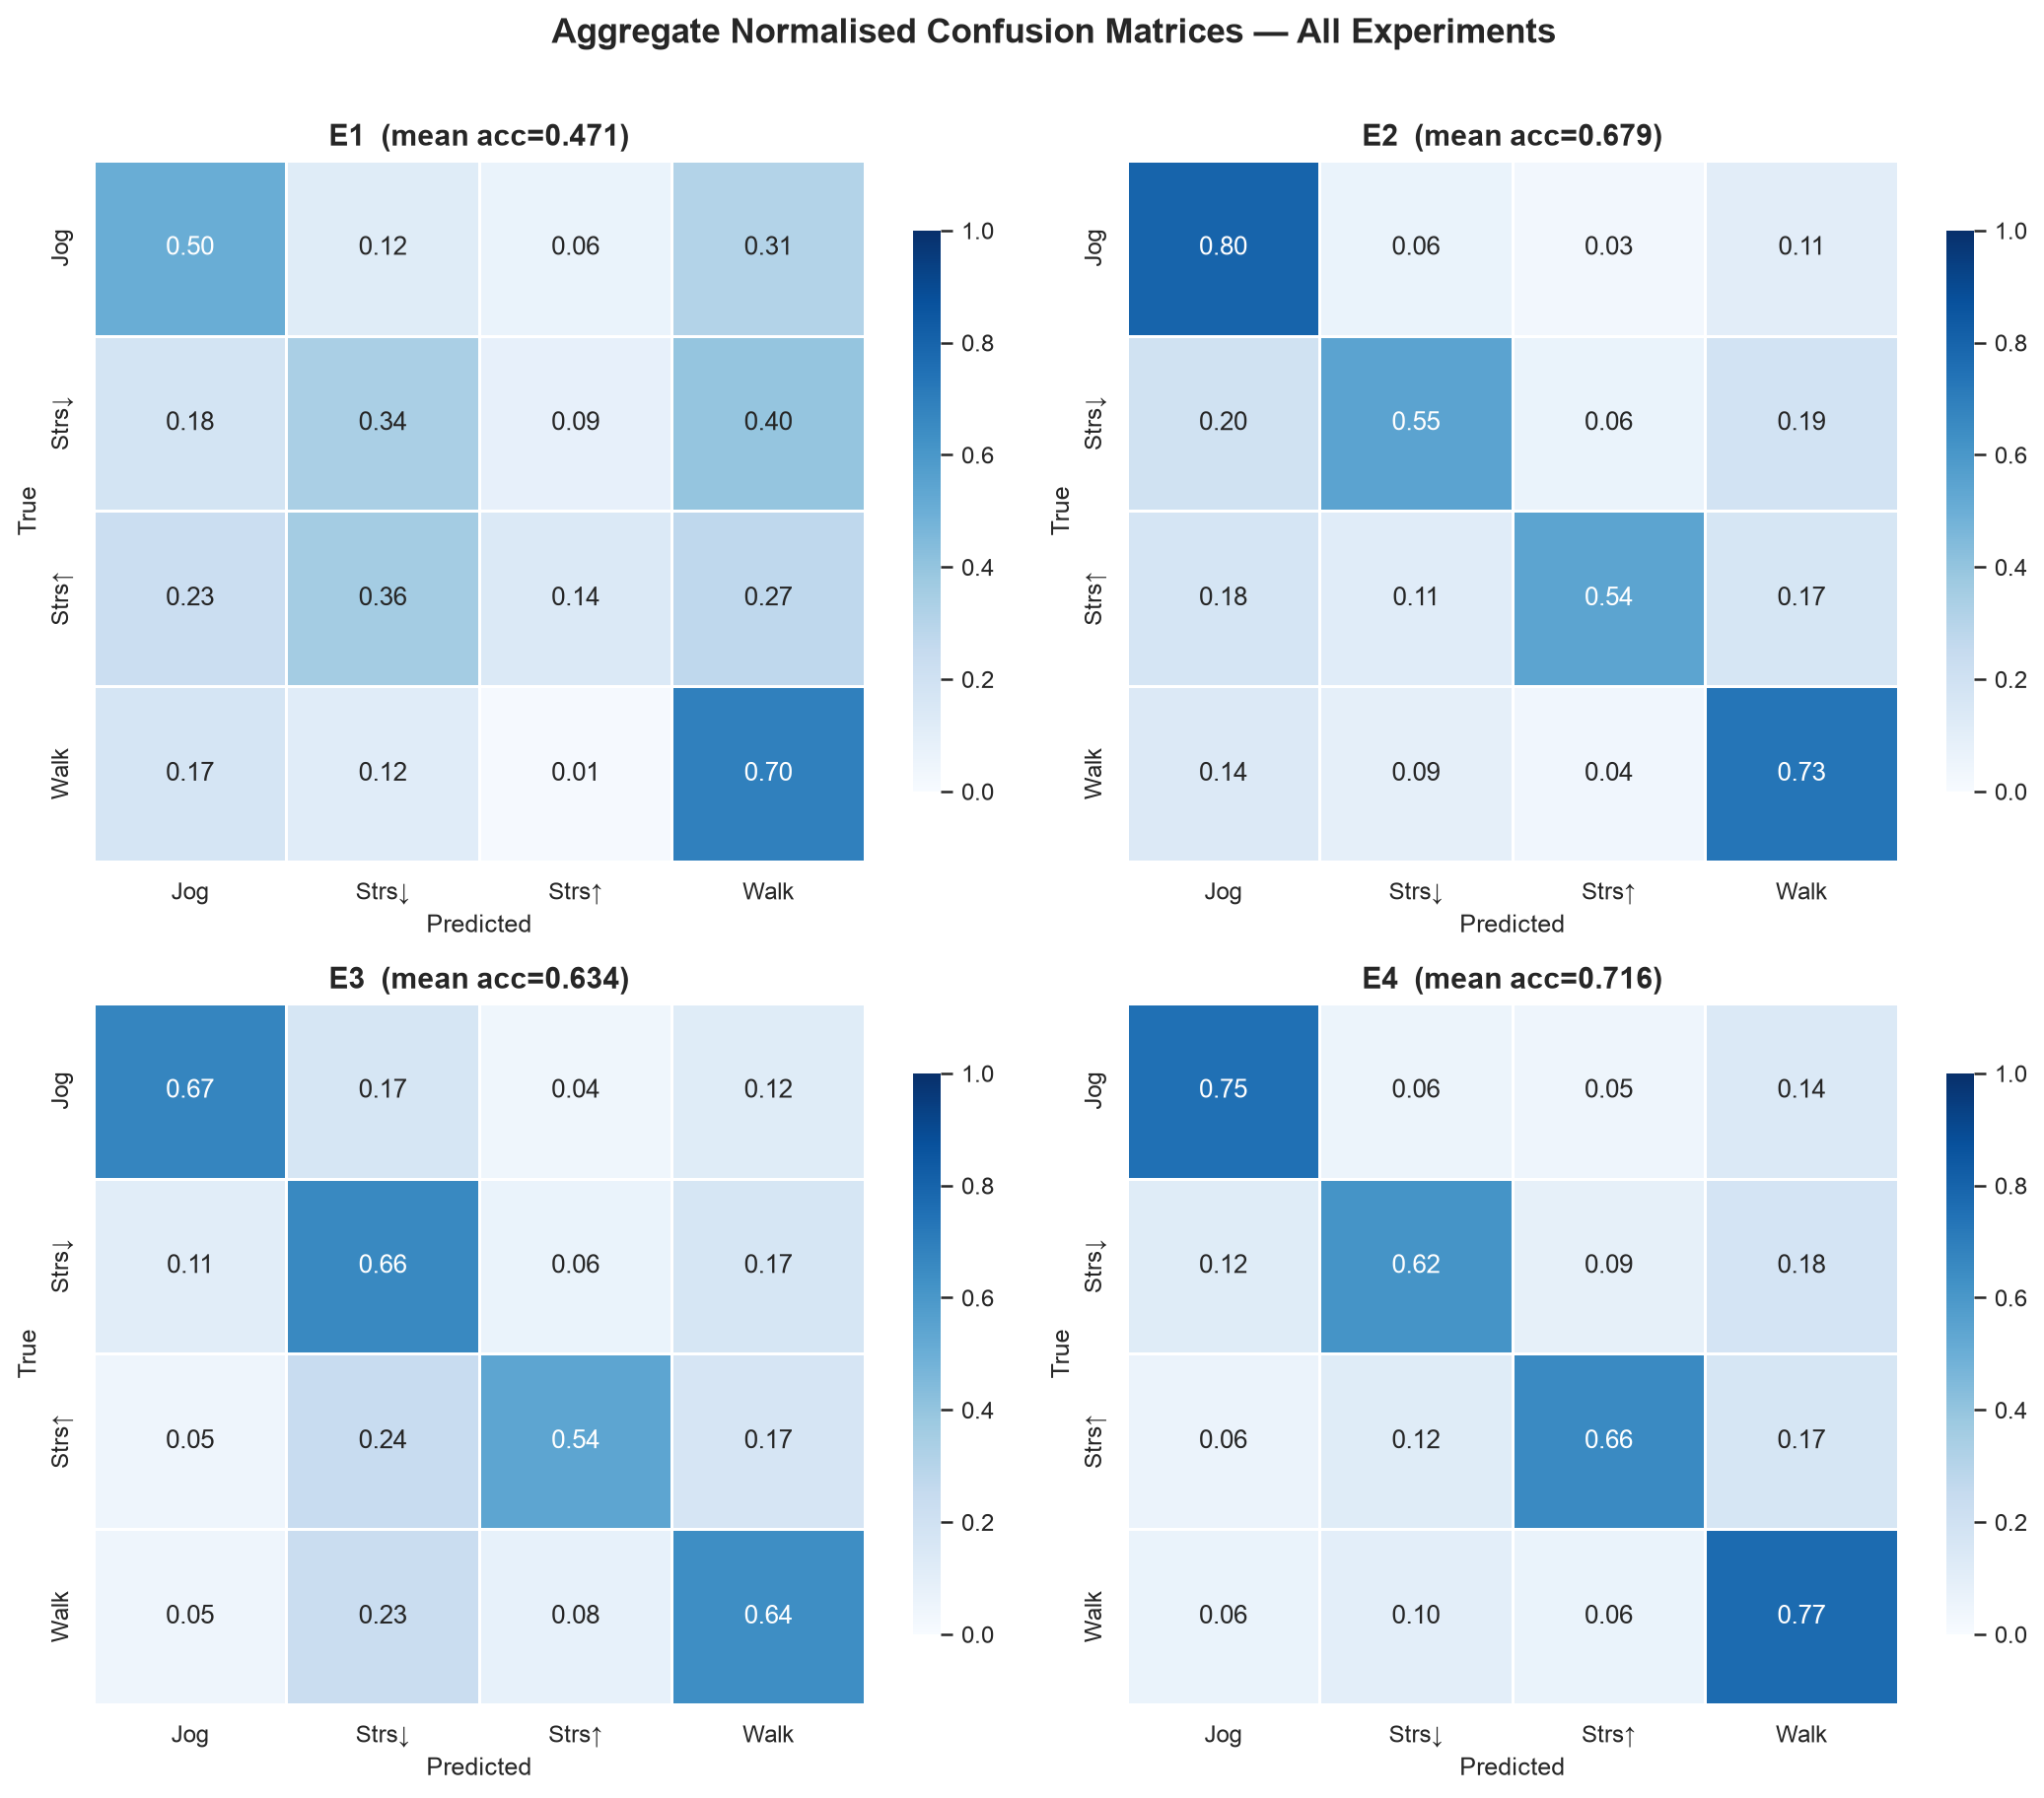
\includegraphics[width=\linewidth]{figures/cm_all_experiments.png}
\caption{Row-normalized aggregate confusion matrices for all four
conditions, pooled across all nine LOSO folds. Diagonal entries equal
the per-class recall values underlying Table~\ref{tab:per-class-f1}.}
\label{fig:confusion-matrices}
\end{figure}

\subsection{Fold-Level Analysis}
\label{subsec:results-fold-level}

Fig.~\ref{fig:accuracy-folds} shows per-fold accuracy for all four
conditions. Fold-to-fold variability differs substantially by
condition: E2's nine folds span the narrowest range (0.598--0.799,
std $0.063$), while E1 (0.250--0.688) and E3 (0.405--0.799) are
both far more variable, and E3's distribution is visibly bimodal,
with folds 1, 2, 6, and 9 all above 0.69 and folds 3, 4, 5, and 8
between 0.40 and 0.64 rather than spread continuously between the
two. E4 is comparatively tight (seven of nine folds between 0.68 and
0.82) except for one clear outlier at $0.540$.

That outlier is fold 3, held out for subject 3, and the same fold is
also the single lowest-accuracy fold for E1 ($0.250$), E2 ($0.598$),
and E3 ($0.424$): every one of the four conditions reaches its
minimum accuracy on the same held-out subject. Because this pattern
holds across E1 and E2, which share no architecture, no fused
features, and no rate-handling choice, we read it as evidence that
subject 3 is harder to generalize to under this protocol for reasons
independent of modality or fusion strategy, rather than as a
weakness specific to any one condition; we do not have an
independent measurement (for example, of movement style, session
conditions, or sensor placement for this participant) that would let
us attribute this directly to a specific cause, and we do not
speculate further than noting the pattern here.

\begin{figure}[t]
\centering
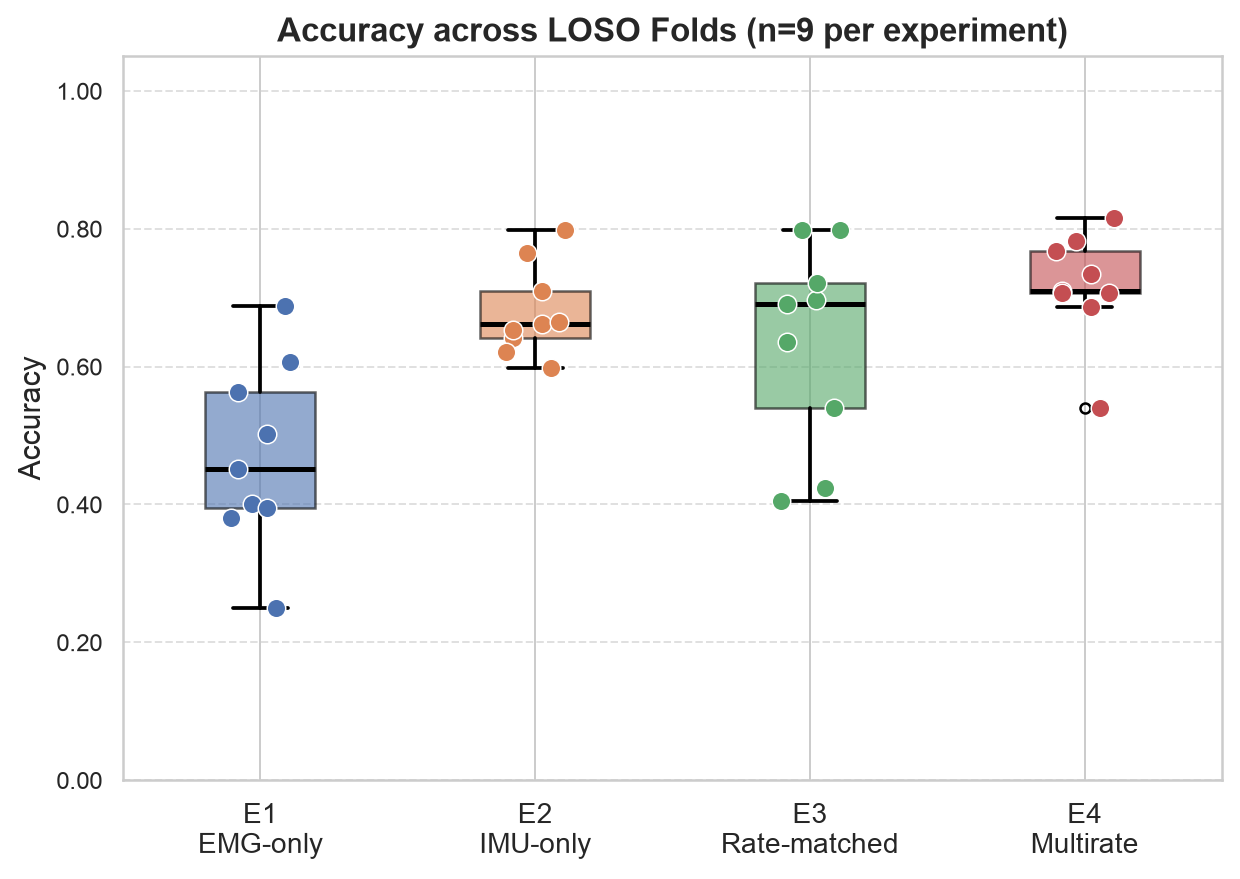
\includegraphics[width=\linewidth]{figures/accuracy_comparison.png}
\caption{Per-fold accuracy for all nine LOSO folds of each condition
($n=9$ points per condition; box shows quartiles, whiskers show the
full range excluding outliers, points show individual folds).}
\label{fig:accuracy-folds}
\end{figure}

\subsection{Statistical Comparison}
\label{subsec:results-statistical}

Table~\ref{tab:statistical-comparisons} reports the paired Wilcoxon
signed-rank test, Holm-Bonferroni-corrected $p$-value, and paired
Cohen's $d$ for all six pairwise comparisons among E1--E4, computed
separately for accuracy and macro F1 as described in Sec.~VI-D
($n=9$ paired folds per comparison). After correction, E1 is
significantly lower than E2 (accuracy and F1), E4 (accuracy and F1),
and E3 (F1 only, $p_{\text{Holm}}=0.031$; the corresponding accuracy
comparison, $p_{\text{Holm}}=0.078$, does not reach significance at
$\alpha=0.05$, so the two metrics do not agree for this pair, and we
report both rather than only the one that is significant). No other
pair, E2 vs.\ E3, E2 vs.\ E4, or E3 vs.\ E4, is statistically
significant after correction for either metric, including the E2
vs.\ E4 and E3 vs.\ E4 comparisons most directly relevant to this
paper's research question. Concretely: E4 achieved the highest
observed mean accuracy and macro F1 of the four conditions
(Sec.~VII-A), but its advantage over E2 (IMU-only) and over E3
(rate-matched fusion) did not reach statistical significance after
multiple-comparison correction, at this sample size ($n=9$ folds).
We report the numerically highest condition and the statistical
result as two separate facts, and we do not describe E4 as having
significantly outperformed E2 or E3 anywhere in this paper, since
Table~\ref{tab:statistical-comparisons} does not support that claim.

\begin{table}[t]
\centering
\small
\caption{Pairwise Wilcoxon signed-rank comparisons ($n=9$ folds),
Holm-Bonferroni-corrected within each metric. $\Delta$ is
mean(A)$-$mean(B); $d$ is paired Cohen's $d$. $^{*}p_{\text{Holm}}<0.05$.}
\label{tab:statistical-comparisons}
\begin{tabular}{llrrr}
\toprule
Pair (A vs.\ B) & Metric & $\Delta$ & $p_{\text{Holm}}$ & $d$ \\
\midrule
E1 vs.\ E2 & Acc & $-0.208$ & $0.039^{*}$ & $-1.71$ \\
           & F1  & $-0.286$ & $0.023^{*}$ & $-2.27$ \\
E1 vs.\ E3 & Acc & $-0.163$ & $0.078$      & $-1.01$ \\
           & F1  & $-0.243$ & $0.031^{*}$ & $-1.49$ \\
E1 vs.\ E4 & Acc & $-0.246$ & $0.023^{*}$ & $-2.14$ \\
           & F1  & $-0.320$ & $0.023^{*}$ & $-2.81$ \\
E2 vs.\ E3 & Acc & $+0.045$ & $0.641$      & $0.46$ \\
           & F1  & $+0.043$ & $0.652$      & $0.43$ \\
E2 vs.\ E4 & Acc & $-0.037$ & $0.148$      & $-0.69$ \\
           & F1  & $-0.034$ & $0.164$      & $-0.70$ \\
E3 vs.\ E4 & Acc & $-0.082$ & $0.082$      & $-0.67$ \\
           & F1  & $-0.076$ & $0.258$      & $-0.71$ \\
\bottomrule
\end{tabular}
\end{table}

% ============================================================
% VIII. DISCUSSION
% ============================================================
\section{Discussion}
\label{sec:discussion}

This paper set out to answer a narrow empirical question (Sec.~I,
Sec.~III): under a leakage-controlled, strictly participant-independent
evaluation of SDALLE, does processing EMG and IMU at their own native
sampling rates through separate branches (E4) change recognition
performance relative to unimodal baselines (E1, E2) and to the
rate-matched fusion approach used by the existing SDALLE benchmark
(E3)? The results in Sec.~VII give a two-part answer rather than a
single verdict. Descriptively, E4 achieved the highest observed mean
accuracy and macro F1 of the four conditions (Sec.~VII-A).
Inferentially, that advantage was statistically confirmed only
against E1: after Holm-Bonferroni correction, E4 was significantly
better than E1 on both metrics, but its numerically higher mean over
E2 and over E3 did not reach significance for either metric
(Sec.~VII-E). The research question is therefore partially supported:
native-rate fusion is not shown to hurt performance relative to
rate-matched fusion or to IMU alone, and it produced the best point
estimate among the four conditions, but this evaluation does not
provide statistical evidence that native-rate processing is the
better choice on SDALLE at this sample size. We treat ``highest
observed mean'' and ``statistically confirmed advantage'' as two
separate facts throughout this discussion, exactly as in
Sec.~VII-E, and we do not collapse them into a single claim of
superiority.

The clearest and most statistically robust finding is that IMU alone
substantially and significantly outperforms EMG alone (E1 vs.\ E2,
both metrics, Table~\ref{tab:statistical-comparisons}), and every
condition that includes IMU outperforms E1 by a wide margin
(Sec.~VII-A). Table~\ref{tab:per-class-f1} and
Fig.~\ref{fig:confusion-matrices} suggest a plausible explanation
rather than a demonstrated mechanism: EMG-only recall for
\texttt{Stairs\_up} is only $0.143$, with most misclassified windows
predicted as \texttt{Stairs\_down} or, more strikingly, as walking,
which is consistent with surface EMG amplitude in this dataset being
a comparatively weak discriminator between locomotion modes that
involve broadly similar overall muscular effort but different limb
kinematics, a limitation the SDALLE dataset paper's own authors also
attribute their weaker EMG-channel accuracies to
\cite{el-khoreby2025sdalle}. IMU, by directly measuring limb
orientation and acceleration, appears better matched to distinguishing
activities that differ mainly in movement trajectory than to
distinguishing them from muscular activation alone, at least at the
window length and architecture used here. This is offered as a
plausible reading of the confusion pattern, not as a general claim
about EMG's usefulness for locomotion recognition under other window
lengths, feature representations, or channel placements.

Whether EMG adds measurable value once IMU is already available is
less clear-cut. Rate-matched fusion (E3) did not significantly
outperform IMU alone ($p_{\text{Holm}}=0.641$ accuracy, $0.652$ F1
for E2 vs.\ E3), and although E3's mean accuracy is nominally lower
than E2's despite adding a modality, we read this as evidence of no
measurable difference rather than evidence that adding EMG hurts,
given how wide E3's fold-to-fold spread is (Sec.~VII-D). Native-rate
fusion (E4) shows a numerically consistent edge over E2 on both
metrics, and unlike E3, this edge coexists with a fold-to-fold spread
that is no wider than E2's own (Sec.~VII-D), which is at least
consistent with native-rate processing preserving usable EMG
information that rate-matched downsampling discards, echoing the
open question raised by the existing SDALLE benchmark
\cite{farouk2026sdalle}. This is a consistency observation, however,
not a statistical demonstration: the E2-vs-E4 comparison itself does
not reach significance for either metric ($p_{\text{Holm}}=0.148$
accuracy, $0.164$ F1), so this evaluation cannot conclude that EMG,
processed at native rate or otherwise, measurably improves on
IMU-only recognition for this dataset and protocol; it can only say
that native-rate fusion produced the best point estimate and showed
no within-fold cost to adding EMG of the kind visible in E3.

The comparison most directly relevant to this paper's contribution,
native-rate versus rate-matched fusion (E3 vs.\ E4), shows a similar
pattern: E4's mean accuracy is $0.082$ higher than E3's and its mean
macro F1 is $0.076$ higher, yet neither difference survives Holm
correction ($p_{\text{Holm}}=0.082$ accuracy, $0.258$ F1). Part of the
explanation is visible directly in Sec.~VII-D: E3's nine folds are
not merely more variable than E4's, they are visibly bimodal, with
four folds performing comparably to E4 and four performing far worse,
which is exactly the kind of high within-condition variance that a
paired test with only nine folds has limited power to distinguish
from a true, smaller, more uniform effect. A second, structural
reason not to attribute this comparison to rate-handling alone is the
capacity asymmetry already flagged in Sec.~V-E: E4's dual-branch
architecture has 330{,}052 trainable parameters against E3's
177{,}732, roughly 1.86 times as many, so any advantage E4 shows
could in principle reflect its larger effective capacity rather than,
or in addition to, the benefit of preserving each modality's native
sampling rate; this evaluation was not designed to separate those two
effects, and doing so would require an E3 variant with matched
capacity, which we did not train and do not claim results for.

More generally, the absence of significance for the E2-vs-E4 and
E3-vs-E4 comparisons should not be read as evidence that native-rate
fusion makes no difference. At $n=9$ paired folds, this design has
limited statistical power to detect effects of the size observed here
(paired Cohen's $d$ of $-0.67$ to $-0.71$ for E3 vs.\ E4 and $-0.69$
to $-0.70$ for E2 vs.\ E4, both in the medium-to-large range by
conventional benchmarks despite not reaching significance after
correction), and a non-significant result at this sample size is
properly read as inconclusive rather than as a null finding. We
report the absence of significance plainly because the goal of this
paper is an honest evaluation-protocol result, not a claim calibrated
to look stronger than the data support.

The single most consistent pattern in the fold-level results
(Sec.~VII-D) is that all four conditions, including the two, E1 and
E2, that share no architecture, no fused features, and no
rate-handling choice, reach their minimum accuracy on the same
held-out fold, subject 3. This cross-condition agreement suggests
that subject-to-subject variability in this dataset, for reasons this
evaluation cannot identify from the data available (possible
candidates include movement style, sensor placement consistency, or
session-specific factors, none of which we measured independently),
may be as consequential for participant-independent performance as
the choice of modality or fusion strategy, at least for this one
participant. This observation is itself an argument for the kind of
participant-independent evaluation this paper reports: a window-level,
non-participant-grouped split, of the kind used for the existing
SDALLE benchmark's headline numbers \cite{farouk2026sdalle}, would not
expose a hard-to-generalize-to subject at all, since windows from that
subject would appear in both the training and test partitions.

These findings relate directly to the two future-work directions the
existing SDALLE benchmark identifies explicitly: participant-independent
evaluation and native- or multi-rate fusion that retains
higher-frequency EMG content \cite{farouk2026sdalle}. Implementing
both changes the picture substantially: overall accuracies in this
evaluation ($0.47$--$0.72$ across conditions,
Table~\ref{tab:overall-performance}) are far below the approximately
99\% reported for attention-enhanced CNN-LSTM models under the
benchmark's window-level split, a gap consistent with, though not a
direct measurement of, the leakage effect the benchmark's own authors
describe for their protocol, and consistent with the broader
literature's documented concern that subject-dependent splits inflate
apparent performance for wearable-sensor activity recognition
\cite{rehman2024validation, cai2025generalizablehar}. We do not claim
this comparison isolates leakage as the sole cause of the gap, since
the two evaluations also differ in architecture, windowing, and
training protocol, but the direction and magnitude of the difference
are consistent with what leakage-sensitive evaluations of similar
tasks have reported elsewhere. For multimodal biomedical and
wearable-sensor recognition more broadly, if the pattern observed
here generalizes beyond SDALLE, and we make no claim that it does
without further evidence on other datasets, it would suggest that
under participant-independent evaluation, the choice of which
modality to weight more heavily (here, IMU over EMG) may matter more
than the specific engineering choice of how to reconcile their
sampling rates during fusion. Establishing that generalization is
outside what a single nine-subject dataset can support; we present it
here as a hypothesis raised by this evaluation, not a conclusion it
establishes.

% ============================================================
% IX. LIMITATIONS
% ============================================================
\section{Limitations}
\label{sec:limitations}

Several limitations bound how far the findings in Sec.~VII and
Sec.~VIII should be generalized, and we state them explicitly rather
than leave them implicit.

The leave-one-subject-out protocol yields exactly nine paired folds
per condition, the maximum available given SDALLE's cohort size, and
this cannot be increased without a different or larger dataset. As
discussed in Sec.~VIII, this limits the paired Wilcoxon test's power
to detect effects of the size observed for the E2-vs-E4 and E3-vs-E4
comparisons, both of which show medium-to-large paired Cohen's $d$
(Table~\ref{tab:statistical-comparisons}) without reaching
significance after Holm-Bonferroni correction. The non-significant
results for these two comparisons should be read as inconclusive at
this sample size, not as evidence that no true difference exists.

SDALLE records nine healthy adult volunteers performing four
discrete, instructed locomotion activities under controlled recording
conditions (Sec.~II-E, Sec.~IV); it is not a continuous, free-living
recording, and it does not include clinical populations such as
stroke survivors, prosthetic or orthotic users, or older adults with
mobility impairment. Nothing in this paper's results should be
extrapolated to those populations, or to unstructured real-world
activity monitoring, without separate validation, and, as stated in
Sec.~I, this study makes no claim of clinical utility or deployment
readiness.

Two discrepancies identified during our own audit of the raw SDALLE
files (Sec.~II-E, Sec.~IV-A) remain unresolved in this manuscript
rather than adjudicated. The dataset paper's stated protocol implies
360 trials, one fewer than the 361 trial files our audit located,
traced to an extra walking trial for Subject~8 (Sec.~IV-D); and the
dataset paper's description of a custom Raspberry-Pi-relayed sensor
module does not match the DELSYS Trigno platform named in the later
benchmark paper. We do not have independent evidence to resolve
either discrepancy and report both as open provenance questions
rather than as data-quality defects.

Model capacity is not held equal across the four conditions. As noted
in Sec.~V-E, E4's dual-branch architecture has 330{,}052 trainable
parameters, 1.86 times E3's 177{,}732 and 2.11 times E1's 156{,}228,
because E4 instantiates two complete encoders rather than one. Any
performance advantage attributed to E4 in Sec.~VII and Sec.~VIII
could therefore reflect its larger capacity in addition to, or
instead of, the benefit of native-rate processing specifically; this
evaluation was not designed to separate the two, and doing so would
require training a capacity-matched E3 variant, which is outside the
scope of this paper.

E1's absolute accuracy is low (mean $0.471$) and highly variable
across folds (range $0.250$--$0.688$, Sec.~VII-D), with particularly
weak recall for \texttt{Stairs\_up} ($0.143$, Sec.~VII-B). This is
consistent with, but does not by itself prove, a genuine limit on how
discriminative these EMG channels are for this task; we did not
explore EMG-specific architectural variants, alternative feature
representations (for example, time-frequency or envelope-based
features rather than raw windowed signal), or channel-selection
strategies, any of which could plausibly change E1's absolute
performance without affecting the E3-vs-E4 comparison this paper is
centered on.

Every (condition, fold) combination was trained once, at a fixed
random seed (Sec.~VI-C), not repeated across multiple seeds. We
therefore cannot fully separate training-run-to-run variance from
genuine subject-to-subject (fold-to-fold) variance in the results
reported in Sec.~VII-D; some part of the observed spread, including
E3's bimodal distribution, could in principle reflect training
stochasticity rather than subject difficulty alone, though the
cross-condition agreement on subject 3 as the hardest fold
(Sec.~VII-D) is not easily explained by single-run training noise
alone, since it recurs independently across four differently
initialized and differently architected models.

All four conditions share one deliberately compact convolutional
architecture family (Sec.~V-E), chosen to hold architecture fixed
across conditions rather than to search for the best-performing
model; the existing SDALLE benchmark evaluates sixteen architectures
\cite{farouk2026sdalle}, and we make no claim that our specific CNN's
absolute numbers represent the best achievable performance under any
of the four input conditions, only that comparisons between
conditions are not confounded by using different architectures for
different conditions.

Finally, E4's per-fold training time was measured at roughly two to
three hours against tens of seconds for E2 and E3 and a few hundred
seconds for E1 (Sec.~VI-E). We report this because it is directly
measurable and may matter for anyone reproducing this work, but we
did not isolate its cause and do not claim it reflects the general
computational cost of native-rate fusion.

% ============================================================
% X. CONCLUSION
% ============================================================
\section{Conclusion}
\label{sec:conclusion}

This paper reported a controlled, leakage-audited,
participant-independent re-evaluation of the SDALLE lower-limb
locomotion dataset, comparing EMG alone (E1), IMU alone (E2), EMG-IMU
fusion after resampling EMG to the IMU rate (E3), and EMG-IMU fusion
with each modality processed at its own native sampling rate through
separate branches (E4), under identical nine-fold
leave-one-subject-out splits. Consistent with the framing in Sec.~III,
this is an empirical reproducibility and evaluation-protocol study,
not a new-architecture contribution, and its conclusions follow
directly from Sec.~VII rather than from any claim asserted in
advance.

Three findings summarize the evidence. First, IMU alone significantly
and substantially outperforms EMG alone under this protocol
(Table~\ref{tab:statistical-comparisons}), and every fusion condition
inherits this advantage over EMG alone. Second, native-rate fusion
(E4) achieved the highest observed mean accuracy ($0.716 \pm 0.074$)
and macro F1 ($0.698 \pm 0.073$) of the four conditions, and was
statistically significantly better than EMG alone on both metrics,
but its advantage over IMU alone (E2) and over rate-matched fusion
(E3) did not reach statistical significance after Holm-Bonferroni
correction at $n=9$ paired folds. Third, a single held-out subject
(subject 3) produced the lowest accuracy for all four conditions, a
pattern that recurs across architecturally unrelated models and
points to subject-level variability, rather than modality or fusion
choice, as a substantial source of the remaining error under
participant-independent evaluation.

Taken together, these results directly implement the two directions
the existing SDALLE benchmark study identifies as necessary future
work, participant-independent evaluation and native-rate multimodal
fusion \cite{farouk2026sdalle}, and show that, once both are applied,
absolute performance on SDALLE is far more modest than the
window-level-split numbers previously reported for this dataset.
Native-rate fusion is not shown to hurt performance relative to the
alternatives evaluated here, and it produced the best point estimate
among them, but this study does not provide statistical evidence, at
this sample size, that native-rate processing is the better choice on
SDALLE; we report this as an open question rather than resolve it,
and we do not describe E4 as having significantly outperformed E2 or
E3 anywhere in this paper. Future work following directly from the
limitations in Sec.~IX includes a capacity-matched ablation to
separate the effect of native-rate processing from E4's larger
parameter count, evaluation on a larger or second lower-limb EMG-IMU
cohort to increase statistical power beyond nine subjects, and
EMG-specific architectural or feature-representation choices that
might change E1's comparatively weak absolute performance without
altering the core native-rate-versus-rate-matched comparison this
paper is centered on.

% ============================================================
% CODE AND DATA AVAILABILITY
% ============================================================
\section*{Code and Data Availability}
\label{sec:availability}

The SDALLE dataset is publicly available from Zenodo under a
Creative Commons Attribution 4.0 International (CC-BY-4.0) license
(DOI: 10.5281/zenodo.14841611) \cite{sdalle2025zenodo}. Raw data are
not redistributed in the accompanying repository; a download script
referencing the Zenodo DOI is provided instead.

All 36 trained model checkpoints (E1--E4, 9 LOSO folds each)
underlying Sec.~VII were retrained under the corrected protocol
described in Sec.~VI-A and Sec.~VI-C, with SHA-256 checksums recorded
for every checkpoint (\texttt{results/final\_results\_checksums.sha256})
and verified against those checksums before evaluation
(\texttt{run\_evaluation.py}, Sec.~VI-D), and a full copy of the
training outputs was preserved immediately after training, before
evaluation was run, so that every number in Sec.~VII can be traced
back to a specific, integrity-checked model file rather than to a
result that could have been silently altered between training and
evaluation.

\todo{Insert the public GitHub repository URL once the code
repository is created and populated. Confirm the repository includes
preprocessing scripts, the leave-one-subject-out splitting logic,
fixed random seeds, a single reproducible entry-point script, the
saved per-fold window-index lists used for the leakage audit, and
\texttt{run\_evaluation.py} together with the checksum and
statistical-testing artifacts referenced above.}

% ============================================================
% DECLARATIONS
% ============================================================
\section*{Declarations}
\label{sec:declarations}

\textbf{Funding.} \todo{State whether this work received external
funding (e.g., a departmental or institutional grant) or none. Not
yet confirmed by the authors; not assumed by this manuscript.}

\textbf{Conflict of Interest.} \todo{The authors must confirm
whether they have any competing financial or non-financial interests
to declare. Not yet confirmed; not assumed by this manuscript.}

\textbf{Ethics Approval.} No new data involving human participants
were collected for this study. All experiments reported here
re-analyze the publicly released, de-identified SDALLE dataset
\cite{sdalle2025zenodo, el-khoreby2025sdalle}, which was collected and
released by its original authors; ethical approval and participant
consent for the original data collection are the responsibility of,
and are reported by, the SDALLE dataset's original publication
\cite{el-khoreby2025sdalle}, not by the present authors.

\textbf{Data Availability.} See ``Code and Data Availability'' above.

\textbf{Author Contributions.} \todo{State each author's specific
contribution (e.g., conceptualization, methodology, software, formal
analysis, writing, supervision), to be agreed and confirmed by both
authors before submission.}

% ============================================================
% REFERENCES
% ============================================================
\bibliographystyle{IEEEtran}
\bibliography{references}

\end{document}
